% ==============================================================================
% CAPÍTULO 5 - IMPLEMENTAÇÃO E ORQUESTRAÇÃO DO ECOSSISTEMA OFICINA MASTER
% ==============================================================================

\chapter{Implementação e Orquestração do Ecossistema Oficina Master}
\label{cap:desenvolvimento}

Este capítulo detalha a implementação técnica do Oficina Master, examinando
as decisões de engenharia adotadas para resolver os desafios inerentes a um
ecossistema \textit{Software as a Service} (SaaS) escalável e multi-tenant.
O desenvolvimento foi orientado por dois princípios fundamentais: a separação
rigorosa de responsabilidades entre camadas de domínio e infraestrutura, e o
uso estratégico de padrões de projeto que garantem a manutenibilidade e a
resiliência do sistema frente ao crescimento contínuo de instâncias isoladas.
Cada decisão técnica aqui documentada reflete um compromisso com a
sustentabilidade arquitetural do produto a longo prazo, priorizando a
rastreabilidade, a idempotência dos processos automatizados e a observabilidade
centralizada do ecossistema.


% ------------------------------------------------------------------------------
\section{Macro Arquitetura e Estratégia de Isolamento de Dados}
% ------------------------------------------------------------------------------

A fundação do Oficina Master é uma arquitetura orientada a serviços que eleva
o isolamento de dados ao status de requisito não-funcional primário. A decisão
arquitetural central foi a adoção do padrão \textbf{Database-per-Tenant}, no
qual cada locatário (\textit{tenant}) possui sua própria instância lógica de
banco de dados, inteiramente segregada das demais.

A adoção desse padrão, em detrimento de abordagens alternativas como o
\textit{Shared Schema} (múltiplos tenants na mesma base, separados por
identificador de coluna) ou o \textit{Shared Database, Separate Schema} (bases
compartilhadas com schemas isolados), foi uma escolha deliberada com implicações
diretas na segurança e na operabilidade. Em um modelo de oficinas mecânicas,
os dados de clientes, veículos e transações financeiras possuem natureza
sensível e estão sujeitos a regulamentações de privacidade. O isolamento físico
elimina classes inteiras de vulnerabilidade, como vazamentos por falhas de
predicados em consultas (ausência de cláusula \texttt{WHERE tenant\_id = ?}) e
simplifica drasticamente os processos de backup granular e recuperação de
desastres por cliente.

\begin{figure}[htb]
    \caption{\label{fig:arquitetura_geral}Macro Arquitetura do Ecossistema Oficina Master}
    \centering
    \begin{tikzpicture}[node distance=2cm, auto, >=latex']
      \node [draw, rectangle, fill=blue!10, text width=3cm, align=center]
        (master_app) {Interface Master\\(Vue.js 3)};
      \node [draw, rectangle, fill=green!10, text width=3cm, align=center,
        below=2.5cm of master_app]
        (master_api) {API Central\\(Laravel 12)};
      \node [draw, cylinder, fill=red!10, text width=2cm, align=center,
        left=3cm of master_api, shape border rotate=90,
        minimum height=1.8cm]
        (db_master) {DB Master\\(Central)};
      \node [draw, cylinder, fill=yellow!10, text width=1.5cm, align=center,
        below=5cm of master_api, xshift=-3cm, shape border rotate=90,
        minimum height=1.6cm]
        (db_t1) {DB T1};
      \node [draw, cylinder, fill=yellow!10, text width=1.5cm, align=center,
        below=5cm of master_api, shape border rotate=90,
        minimum height=1.6cm]
        (db_t2) {DB T2};
      \node [draw, cylinder, fill=yellow!10, text width=1.5cm, align=center,
        below=5cm of master_api, xshift=3cm, shape border rotate=90,
        minimum height=1.6cm]
        (db_tn) {DB Tn};
      \draw [<->] (master_app) -- (master_api);
      \draw [<->] (master_api) -- (db_master);
      \draw [->]  (master_api) -- (db_t1);
      \draw [->]  (master_api) -- (db_t2);
      \draw [->]  (master_api) -- (db_tn);
      \node [draw, rectangle, dashed, fill=white, text width=8cm, align=center,
        below=3cm of master_api, minimum height=1.2cm]
        (tenants_zone) {Ecossistema de Tenants};
    \end{tikzpicture}
    \legend{Fonte: Própria do autor (2026).}
\end{figure}

Conforme ilustrado na \autoref{fig:arquitetura_geral}, o Hub Master atua como
núcleo de orquestração do ecossistema. A API Central, implementada em
\textit{Laravel} 12, mantém as credenciais e os metadados necessários para
gerenciar cada instância de banco de dados individual. O banco de dados Master,
por sua vez, é exclusivamente dedicado ao armazenamento de dados de
orquestração: metadados dos tenants, logs de acesso consolidados e definições
dos planos de assinatura. Esta separação de responsabilidades garante que falhas
isoladas em uma instância de cliente --- sejam elas decorrentes de corrupção de
dados, sobrecarga de queries ou manutenção planejada --- não comprometam a
integridade ou a disponibilidade do restante do ecossistema, satisfazendo o
princípio de \textit{blast radius} mínimo em arquiteturas de alta
disponibilidade.


% ------------------------------------------------------------------------------
\section{Organização do Projeto e Padrões de Implementação}
% ------------------------------------------------------------------------------

O projeto foi estruturado seguindo as convenções modernas do \textit{framework
Laravel}, estendendo sua funcionalidade nativa para suportar o multi-tenancy
dinâmico. A organização do código é reflexo direto da separação entre lógica
de domínio e infraestrutura, princípio fundamental da Arquitetura Limpa
(\textit{Clean Architecture}) proposta por \citeonline{martin2017}.

\subsection{Estrutura de Pastas e Namespaces}

A lógica de negócio foi centralizada na pasta \texttt{app/Services}, organizada
em domínios coesos e de responsabilidade única:

\begin{itemize}
    \item \texttt{App\textbackslash{}Services\textbackslash{}Tenants}: Contém o
    \texttt{TenantDatabaseService}, responsável por toda a manipulação de
    infraestrutura de bancos de dados, incluindo criação, inicialização e
    teardown de instâncias;

    \item \texttt{App\textbackslash{}Services\textbackslash{}Licencas}: Agrupa
    as regras de validação, renovação e controle de status de assinaturas,
    isolando completamente a lógica de negócio de licenciamento da camada de
    persistência;

    \item \texttt{App\textbackslash{}Http\textbackslash{}Controllers\textbackslash{}Api}:
    Controladores enxutos (\textit{Lean Controllers}) que atuam exclusivamente
    como orquestradores de requisições, delegando toda a lógica de negócio aos
    serviços de domínio correspondentes.
\end{itemize}

Esta organização tem impacto direto na testabilidade do sistema. Ao desacoplar
os serviços de domínio dos controladores HTTP, torna-se possível escrever testes
unitários para cada serviço de forma isolada, sem a necessidade de instanciar
o contexto completo da aplicação web. A injeção de dependências gerenciada pelo
contêiner IoC (\textit{Inversion of Control}) do Laravel viabiliza a
substituição de implementações concretas por dublês de teste (\textit{mocks} e
\textit{stubs}), elevando a confiabilidade da suíte de testes.

\subsection{Camada de Modelagem: Eloquent e Relacionamentos de Domínio}

O banco de dados Master utiliza modelos Eloquent para gerenciar a orquestração
do ecossistema. O modelo \texttt{Tenant} é a entidade central deste domínio,
armazenando não apenas as configurações de conexão (host, database, username),
mas também o estado operacional de cada instância e seu histórico de eventos.
A relevância desta entidade transcende o simples mapeamento de uma tabela: ela
é o ponto de convergência entre infraestrutura, licenciamento e faturamento.

Relacionamentos Eloquent complexos foram modelados para vincular cada
\texttt{Tenant} a uma \texttt{Empresa} (entidade de negócio) e às suas
respectivas \texttt{Licencas}. Esta estrutura relacional permite a execução de
consultas analíticas agregadas --- como a identificação de tenants com licenças
próximas ao vencimento ou com crescimento acelerado de armazenamento ---
diretamente na camada de modelo, sem a necessidade de lógica de agregação
dispersa nos controladores. A decisão de normalizar esta relação em três
entidades distintas (\texttt{Tenant}, \texttt{Empresa}, \texttt{Licenca}),
em vez de consolidá-las em uma única tabela, foi motivada pelo princípio da
responsabilidade única e pela antecipação de requisitos futuros, como a
possibilidade de um mesmo grupo empresarial gerenciar múltiplos tenants.


% ------------------------------------------------------------------------------
\section{Provisionamento Automatizado e Orquestração de Instâncias}
% ------------------------------------------------------------------------------

O provisionamento de novas empresas parceiras no ecossistema do Oficina Master
constitui um dos processos de maior criticidade operacional da plataforma.
Manualmente, este fluxo envolveria a execução sequencial e propensa a erros de
comandos de banco de dados, configurações de acesso e inicialização de dados
--- um processo inviável na escala proposta pelo produto. A solução implementada
automatiza integralmente esta sequência, seguindo o princípio de
\textbf{idempotência}: cada etapa do fluxo pode ser reexecutada sem produzir
efeitos colaterais indesejados caso parcialmente concluída.

O fluxo de trabalho de provisionamento, representado formalmente no diagrama de
atividades da \autoref{fig:fluxo_provisionamento}, evidencia a natureza
transacional do processo. Cada etapa da cadeia é uma operação atômica; a
falha em qualquer ponto aciona o mecanismo de compensação (\textit{rollback})
sobre o banco de dados Master, revertendo os metadados registrados e garantindo
que nenhuma instância parcialmente inicializada persista no ecossistema.

\begin{figure}[htb]
    \caption{\label{fig:fluxo_provisionamento}Diagrama de Atividades: Provisionamento Automatizado de Nova Instância}
    \centering
    \begin{tikzpicture}[
        node distance=1.4cm,
        auto,
        block/.style={draw=blue!60, fill=blue!5, rectangle, text width=7cm, align=left, minimum height=0.9cm, rounded corners=4pt, font=\small},
        decision/.style={draw=orange!60, fill=orange!5, diamond, aspect=2.2, text width=2.2cm, align=center, minimum height=0.8cm, font=\small},
        failed/.style={draw=red!60, fill=red!5, rectangle, text width=4.5cm, align=center, minimum height=0.9cm, rounded corners=4pt, font=\small},
        success/.style={draw=green!60, fill=green!5, rectangle, text width=4.5cm, align=center, minimum height=1.1cm, rounded corners=4pt, font=\small},
        startstop/.style={draw=black!50, fill=gray!10, rectangle, minimum height=0.7cm, text width=3.5cm, align=center, rounded corners=8pt, font=\small\bfseries},
        line/.style={draw=black!70, -latex', thick}
    ]
        % Nodes
        \node [startstop] (start) {Início: Requisição};
        \node [block, below=0.6cm of start] (step1) {\textbf{1. Criação do Banco de Dados}\\Executa \texttt{CREATE DATABASE} no servidor de banco de dados};
        \node [decision, below=0.6cm of step1] (check1) {Sucesso?};
        
        \node [block, below=0.6cm of check1] (step2) {\textbf{2. Configuração de Conexão}\\Injeta credenciais de acesso via \texttt{Config::set('database...')}};
        \node [decision, below=0.6cm of step2] (check2) {Sucesso?};
        
        \node [block, below=0.6cm of check2] (step3) {\textbf{3. Importação do Dump Inicial}\\Injeta esquema e tabelas padrão via dump SQL};
        \node [decision, below=0.6cm of step3] (check3) {Sucesso?};
        
        \node [block, below=0.6cm of check3] (step4) {\textbf{4. Injeção do Administrador}\\Cria registro de usuário gestor inicial no tenant};
        \node [decision, below=0.6cm of step4] (check4) {Sucesso?};
        
        \node [success, below=0.8cm of check4] (end) {\textbf{Provisionamento Concluído}\\Instância configurada e ativa};
        \node [startstop, below=0.6cm of end] (end_state) {Fim: Sucesso};
        
        \node [failed, right=2.8cm of check2, yshift=1.2cm] (rollback) {\textbf{Compensação (Rollback)}\\Remove banco de dados criado e limpa metadados do orquestrador};
        \node [startstop, below=0.8cm of rollback] (fail_end) {Fim: Erro};

        % Connections
        \draw [line] (start) -- (step1);
        \draw [line] (step1) -- (check1);
        
        \draw [line] (check1) -- node[left] {Sim} (step2);
        \draw [line] (check1.east) -- node[above] {Não} ++(1.5,0) |- (rollback.west);
        
        \draw [line] (step2) -- (check2);
        \draw [line] (check2) -- node[left] {Sim} (step3);
        \draw [line] (check2.east) -- node[above] {Não} (rollback.west);
        
        \draw [line] (check3) -- node[left] {Sim} (step4);
        \draw [line] (check3.east) -- node[above] {Não} ++(1.5,0) |- (rollback.west);
        
        \draw [line] (step3) -- (check3);
        
        \draw [line] (step4) -- (check4);
        \draw [line] (check4) -- node[left] {Sim} (end);
        \draw [line] (check4.east) -- node[above] {Não} ++(1.5,0) |- (rollback.west);
        
        \draw [line] (end) -- (end_state);
        \draw [line] (rollback) -- (fail_end);
    \end{tikzpicture}
    \legend{Fonte: Própria do autor (2026).}
\end{figure}

A escolha por um fluxo \textbf{síncrono} em detrimento de uma abordagem
assíncrona baseada em filas de mensagens (\textit{message queues}) foi uma
decisão arquitetural consciente. Em um sistema de gestão B2B onde o operador
aguarda ativamente a confirmação do provisionamento, a latência adicional de
poucos segundos é aceitável, ao passo que a complexidade introduzida por um
broker de mensagens (como RabbitMQ ou Laravel Horizon) seria desproporcional
para a escala atual. Esta decisão está documentada como uma dívida técnica
planejada, a ser revisada quando o volume de provisionamentos diários justificar
a adoção de processamento assíncrono.

\subsection{TenantDatabaseService: Motor de Provisionamento e Estratégia de Inicialização}

O componente \texttt{TenantDatabaseService} encapsula a lógica de baixo nível
para criação e inicialização de instâncias, funcionando como a camada de
abstração entre a lógica de orquestração de alto nível e as operações diretas
de banco de dados. A centralização desta responsabilidade em um único serviço,
em vez de distribuí-la pelos controladores, foi motivada pela necessidade de
garantir que qualquer variação futura no processo de provisionamento --- como
a migração para um serviço gerenciado de banco de dados em nuvem --- exija
modificações em um único ponto do sistema.

O método central, \texttt{createAndInitialize}, realiza quatro operações em
sequência controlada. Primeiramente, executa o comando \texttt{CREATE DATABASE}
no servidor de banco de dados alvo, criando a instância lógica. Em seguida,
reconfigura em tempo de execução as conexões do \textit{framework} via
\texttt{Config::set()}, evitando a necessidade de reinicialização da aplicação
ou de arquivos de configuração pré-existentes para cada tenant. A terceira etapa
consiste na injeção do arquivo \texttt{oficina.dump} através do método
\texttt{DB::connection()->unprepared()}, garantindo que toda nova empresa inicie
suas operações com uma estrutura de dados idêntica, validada e livre de
inconsistências de migração incremental. Por fim, as credenciais do
administrador inicial são injetadas diretamente na nova base de dados, tornando
a instância imediatamente operacional sem intervenção manual adicional.

A opção pelo uso de um \textit{dump} SQL pré-validado, em vez da execução
sequencial das \textit{migrations} do Laravel, merece justificativa técnica.
Embora as \textit{migrations} representem a abordagem convencional, sua execução
sequencial sobre bases recém-criadas introduz risco de inconsistência caso
alguma migração intermediária apresente falha. O \textit{dump} garante um estado
inicial determinístico e testado, reduzindo a superfície de falha do
provisionamento.

\subsection{Mecanismo de Rollback e Garantias de Consistência}

A confiabilidade do processo de provisionamento depende criticamente do
comportamento da camada de rollback. Em caso de falha em qualquer das etapas
descritas, a transação aberta no banco de dados Master é revertida
integralmente, eliminando os registros de metadados parcialmente criados.
Contudo, a criação física do banco de dados no servidor MySQL é uma operação
DDL (\textit{Data Definition Language}) que, por definição, não é transacional
na maioria dos motores de banco de dados relacionais. Isso implica que, em
cenários de falha após a criação física mas antes da conclusão do registro de
metadados, o sistema prevê uma rotina de coleta de lixo (\textit{garbage
collection}) que identifica e remove instâncias físicas órfãs --- aquelas
presentes no servidor de banco de dados mas sem correspondência na tabela de
tenants do Master.


% ------------------------------------------------------------------------------
\section{Gestão Centralizada e Hub de Bancos de Dados}
% ------------------------------------------------------------------------------

O monitoramento contínuo de centenas de instâncias de banco de dados impõe
requisitos operacionais que vão muito além das ferramentas convencionais de
administração de banco de dados. Ferramentas como phpMyAdmin ou clientes SQL
genéricos operam sobre uma conexão fixa, exigindo reconexão manual a cada
instância inspecionada. O Oficina Master resolve este problema por meio de
um Hub centralizado com alternância dinâmica de contexto, desenvolvido como
parte integrante da plataforma.

\subsection{Tenant Switching: Alternância Dinâmica de Contexto de Conexão}

O desafio de gerenciar múltiplas conexões de banco de dados em uma única sessão
de aplicação foi resolvido através do padrão \textbf{Tenant Switching}. A
solução abandona o paradigma de conexões fixas configuradas estaticamente no
arquivo \texttt{.env}, adotando em seu lugar uma estratégia de configuração
dinâmica em tempo de execução. O princípio é simples em sua intenção, mas
sofisticado em sua implementação: antes de qualquer operação sobre um tenant
específico, o sistema invalida o cache de conexões existente (\texttt{DB::purge()})
e renegocia os parâmetros da conexão nomeada (\texttt{tenant}) com as
credenciais do banco de dados alvo.

O diagrama de sequência da \autoref{fig:fluxo_conexao} representa formalmente
os atores e as mensagens trocadas neste processo, evidenciando que a operação
de alternância é inteiramente transparente para o administrador: a interface
Vue.js abstrai a complexidade da troca de contexto, apresentando ao usuário
apenas os dados do tenant selecionado.

\begin{figure}[htb]
    \caption{\label{fig:fluxo_conexao}Diagrama de Sequência: Alternância Dinâmica de Contexto de Tenant (\textit{Tenant Switcher})}
    \centering
    \begin{tikzpicture}[
        node distance=2.5cm,
        auto,
        actor/.style={draw=black!70, rectangle, fill=gray!5, text width=3.8cm, align=center, minimum height=1.0cm, rounded corners=3pt, font=\small\bfseries},
        lifeline/.style={draw, gray!60, thick},
        msg/.style={draw=black!90, -latex', thick},
        reply/.style={draw=black!70, -latex', dashed, thick},
        scale=0.95
    ]
        % Entities (lifeline headers - top)
        \node [actor] (ui_top) {UI Master\\(Administrador)};
        \node [actor, right=1.8cm of ui_top] (laravel_top) {Sistema Laravel\\(Service)};
        \node [actor, right=2.5cm of laravel_top] (db_top) {Banco de Dados do Tenant\\(Tenant DB)};

        % Coordinates for vertical lines alignment
        \coordinate (ui_x) at (ui_top.south);
        \coordinate (laravel_x) at (laravel_top.south);
        \coordinate (db_x) at (db_top.south);

        % Y-coordinates
        \def\yStart{-1.0}
        \def\yPurge{-1.8}
        \def\yConfig{-3.0}
        \def\yTest{-4.4}
        \def\yValidate{-5.0}
        \def\yAltStart{-6.2}
        \def\yFailErr{-6.8}
        \def\yFailResp{-7.6}
        \def\yAltSep{-8.4}
        \def\ySuccConfirm{-9.0}
        \def\ySuccLoad{-9.8}
        \def\ySuccResp{-11.2}
        \def\yAltEnd{-12.0}
        \def\yBot{-12.6}

        % Lifeline ends
        \coordinate (ui_bot) at (ui_x |- 0,\yBot);
        \coordinate (laravel_bot) at (laravel_x |- 0,\yBot);
        \coordinate (db_bot) at (db_x |- 0,\yBot);

        % Lifeline headers - bottom
        \node [actor, below=12.6cm of ui_top] (ui_btn) {UI Master\\(Administrador)};
        \node [actor, below=12.6cm of laravel_top] (laravel_btn) {Sistema Laravel\\(Service)};
        \node [actor, below=12.6cm of db_top] (db_btn) {Banco de Dados do Tenant\\(Tenant DB)};

        % Draw Lifelines
        \draw [lifeline] (ui_x) -- (ui_bot);
        \draw [lifeline] (laravel_x) -- (laravel_bot);
        \draw [lifeline] (db_x) -- (db_bot);

        % Activation bars
        % Laravel: Blue from \yStart to \ySuccConfirm, Purple from \ySuccConfirm to \ySuccResp
        \draw [fill=blue!20, draw=blue!50] ([xshift=-0.08cm]laravel_x |- 0,\yStart) rectangle ([xshift=0.08cm]laravel_x |- 0,\ySuccConfirm);
        \draw [fill=purple!20, draw=purple!50] ([xshift=-0.08cm]laravel_x |- 0,\ySuccConfirm) rectangle ([xshift=0.08cm]laravel_x |- 0,\ySuccResp);
        
        % Tenant DB: Green from \yTest to \ySuccConfirm
        \draw [fill=green!20, draw=green!50] ([xshift=-0.08cm]db_x |- 0,\yTest) rectangle ([xshift=0.08cm]db_x |- 0,\ySuccConfirm);

        % Messages
        % 1. Solicitar Troca de Contexto de Tenant (ID)
        \draw [msg] (ui_x |- 0,\yStart) -- node [above, scale=0.8, midway] {Solicitar Troca de Contexto de Tenant (ID)} (laravel_x |- 0,\yStart);

        % 1. Purgar Conexão Existente (DB::purge('tenant'))
        \draw [msg] (laravel_x |- 0,\yPurge) -- ++(1.0,0) coordinate (p1) |- (laravel_x |- 0,\yPurge - 0.8);
        \node [right, scale=0.75, align=left] at (p1 |- 0,\yPurge - 0.4) {Preparar Novo Contexto\\1. Purgar Conexão Existente\\(DB::purge('tenant'))};

        % 2. Definir Nova Configuração (Config::set(config))
        \draw [msg] (laravel_x |- 0,\yConfig) -- ++(1.0,0) coordinate (p2) |- (laravel_x |- 0,\yConfig - 0.8);
        \node [right, scale=0.75, align=left] at (p2 |- 0,\yConfig - 0.4) {2. Definir Nova Configuração\\(Config::set(config))};

        % Testar e Estabelecer Nova Conexão
        \draw [msg] (laravel_x |- 0,\yTest) -- node [above, scale=0.8, midway] {Testar e Estabelecer Nova Conexão} (db_x |- 0,\yTest);

        % Validar Conexão
        \draw [msg] (db_x |- 0,\yValidate) -- ++(1.0,0) coordinate (p3) |- (db_x |- 0,\yValidate - 0.8);
        \node [right, scale=0.75] at (p3 |- 0,\yValidate - 0.4) {Validar Conexão};

        % alt Box
        \draw [draw=black, thick] ([xshift=-0.8cm]ui_x |- 0,\yAltStart) rectangle ([xshift=0.8cm]db_x |- 0,\yAltEnd);
        
        % alt Label Box
        \draw [draw=black, fill=white, thick] 
            ([xshift=-0.8cm]ui_x |- 0,\yAltStart) -- ++(0.7, 0) -- ++(0, -0.35) -- ++(-0.2, -0.1) -- ++(-0.5, 0) -- cycle;
        \node [scale=0.8, font=\bfseries] at ([xshift=-0.45cm, yshift=-0.22cm]ui_x |- 0,\yAltStart) {alt};

        % alternative 1: Failure
        \draw [reply] (db_x |- 0,\yFailErr) -- node [above, scale=0.8, midway] {Erro de Conexão} (laravel_x |- 0,\yFailErr);
        \draw [reply] (laravel_x |- 0,\yFailResp) -- node [above, scale=0.8, midway] {Falha na Troca de Contexto} (ui_x |- 0,\yFailResp);

        % alt Separator Dotted Line
        \draw [dashed, gray!80, thick] ([xshift=-0.8cm]ui_x |- 0,\yAltSep) -- ([xshift=0.8cm]db_x |- 0,\yAltSep);

        % alternative 2: Success
        \draw [reply] (db_x |- 0,\ySuccConfirm) -- node [above, scale=0.8, midway] {Conexão Confirmada} (laravel_x |- 0,\ySuccConfirm);
        
        % 3. Carregar Dados Iniciais
        \draw [msg] (laravel_x |- 0,\ySuccLoad) -- ++(1.0,0) coordinate (p4) |- (laravel_x |- 0,\ySuccLoad - 0.8);
        \node [right, scale=0.75, align=left] at (p4 |- 0,\ySuccLoad - 0.4) {3. Carregar Dados Iniciais};
            
        \draw [reply] (laravel_x |- 0,\ySuccResp) -- node [above, scale=0.8, midway] {Resposta de Sucesso (Contexto Trocado)} (ui_x |- 0,\ySuccResp);

    \end{tikzpicture}
    \legend{Fonte: Própria do autor (2026).}
\end{figure}

Uma implicação arquitetural importante deste padrão é a sua natureza
\textbf{not thread-safe} em ambientes de servidor com workers concorrentes.
Em servidores que utilizam PHP-FPM com múltiplos workers (processos), cada
requisição é tratada de forma isolada em seu próprio processo, o que elimina
o risco de vazamento de contexto entre tenants. Esta garantia de isolamento
por processo é, portanto, uma dependência implícita do modelo de execução do
PHP, e deve ser considerada no planejamento de migração para runtimes
alternativos, como RoadRunner ou Swoole, que operam com workers persistentes
em memória.

\subsection{Telemetria e Observabilidade das Instâncias}

A alternância dinâmica de contexto habilita uma capacidade que vai muito além
da simples execução de queries manuais: permite a coleta sistemática de métricas
de saúde de cada instância, alimentando o painel de observabilidade centralizado
da plataforma. Através da interface Master, o \texttt{DatabaseController}
consolida dados de telemetria por instância: quantidade de tabelas e registros
ativos, espaço em disco ocupado --- discriminado entre dados (\textit{data}) e
índices (\textit{index}) --- e logs de erro com timestamps de última ocorrência.

Esta visibilidade centralizada tem impacto direto na postura operacional da
equipe técnica: em vez de uma abordagem reativa, onde problemas são reportados
por clientes afetados, o sistema habilita uma cultura de monitoramento proativo.
A identificação de crescimento anômalo de tamanho de banco de dados, por exemplo,
pode sinalizar um problema de dados duplicados ou ausência de rotinas de
arquivamento, permitindo intervenção antes que o cliente perceba degradação de
performance.


% ------------------------------------------------------------------------------
\section{Administração de Planos e Licenciamento Flexível}
% ------------------------------------------------------------------------------

A sustentabilidade financeira do ecossistema Oficina Master fundamenta-se em
um modelo de planos altamente configurável, cujo design foi orientado pela
necessidade de suportar diferentes perfis de clientes --- desde oficinas
independentes de pequeno porte até redes de franquias com múltiplas filiais.
A flexibilidade do modelo de licenciamento é, portanto, não apenas uma decisão
comercial, mas uma exigência arquitetural que impacta diretamente a estrutura
de dados e a lógica de controle de acesso da plataforma.

\subsection{Estrutura de Planos e Configuração de Módulos}

Cada plano é representado pela entidade \texttt{Plano}, que armazena em formato
JSON a lista de módulos habilitados para um determinado nível de assinatura.
A adoção do tipo JSON para este atributo, em vez de uma tabela relacional de
associação entre planos e módulos, foi motivada pela natureza altamente variável
da composição de módulos: a criação de uma nova combinação de funcionalidades
não exige alterações no schema do banco de dados, reduzindo o custo de
manutenção e a possibilidade de migrações disruptivas em produção. Os módulos
disponíveis incluem domínios funcionais como Vendas, Estoque, Financeiro e
emissão de Nota Fiscal Eletrônica (NF-e), cada qual com impacto direto nas
permissões de acesso à API do tenant correspondente.

O \texttt{PlanoController} gerencia o ciclo de vida dos modelos de plano,
expondo endpoints para a definição de limites operacionais (número máximo de
usuários simultâneos e cota de armazenamento), controle de precificação e
períodos de renovação, e configuração granular de permissões por módulo.
A separação entre a entidade \texttt{Plano} e a entidade \texttt{Licenca}
é uma distinção semântica fundamental: o plano define \textit{o que} está
disponível; a licença define \textit{para quem} e \textit{por quanto tempo}.

\subsection{Ciclo de Vida do Licenciamento e Controle de Acesso}

A licença ativa de um tenant é o artefato que materializa o contrato comercial
entre a FK Oficina e cada empresa parceira. Seu ciclo de vida compreende quatro
estados: \textit{pendente} (emitida, aguardando ativação), \textit{ativa}
(dentro do período de vigência), \textit{expirada} (prazo encerrado, sem
renovação) e \textit{suspensa} (bloqueada manualmente por intervenção
administrativa). A transição entre esses estados é gerenciada pelo
\texttt{LicencaService} e verificada em cada requisição recebida pela API
do tenant.

O mecanismo de verificação é implementado como um \textit{middleware} do
Laravel, posicionado antes das camadas de autenticação e autorização do tenant.
Esta decisão de design garante que o controle de licenciamento seja
transversal e não possa ser contornado por configurações específicas de rotas
ou controladores. Quando uma licença é identificada como expirada ou suspensa,
a API do tenant retorna um código HTTP \texttt{402 Payment Required} ou
\texttt{403 Forbidden}, respectivamente, acompanhado de uma mensagem estruturada
que a interface do usuário final pode interpretar para exibir um aviso
contextual ao operador da oficina.


% ------------------------------------------------------------------------------
\section{Dashboard Administrativo e Interface Reativa}
% ------------------------------------------------------------------------------

O Dashboard Master representa a síntese operacional de toda a arquitetura
descrita nas seções anteriores: é a camada de apresentação que transforma dados
distribuídos em múltiplas instâncias e domínios em inteligência acionável para
o gestor do ecossistema. Construído com \textit{Vue.js} 3 e consumindo a API
Central do Laravel, o Dashboard atua como o ponto único de verdade (\textit{single
source of truth}) para a tomada de decisões operacionais e estratégicas.

\subsection{KPIs e Métricas Agregadas por Domínio}

O \texttt{DashboardController} realiza a agregação de dados provenientes de
múltiplos domínios do sistema, calculando indicadores-chave de desempenho (KPIs)
que refletem a saúde multidimensional do ecossistema. A organização dos
indicadores em quatro domínios distintos --- saúde da base de clientes, status
de licenciamento, engajamento de uso e saúde financeira --- não é apenas uma
decisão de UX, mas reflete a estrutura de responsabilidades da equipe que opera
a plataforma: cada domínio de KPI corresponde a um fluxo de trabalho diferente,
seja ele de suporte técnico, sucesso do cliente, produto ou faturamento.

O indicador de \textbf{saúde da base de clientes} consolida o quantitativo de
empresas ativas versus inativas, permitindo identificar tendências de churn.
O \textbf{status de licenciamento} apresenta o total de licenças vigentes e
emite alertas sobre vencimentos iminentes, habilitando ações proativas de
renovação. O monitoramento de \textbf{engajamento e uso}, alimentado pelos logs
de acesso (\texttt{AuthAccessLog}), fornece dados de atividade diária por
tenant, possibilitando a identificação de instâncias subutilizadas --- um sinal
precoce de risco de cancelamento. Por fim, a dimensão de \textbf{saúde
financeira} consolida recebíveis e faturamento mensal através do modelo
\texttt{Pagamento}, oferecendo uma visão integrada da performance comercial
do ecossistema.

\begin{figure}[htb]
    \caption{\label{fig:dashboard_interface}\textit{Dashboard} Administrativo: Painel Integrado de KPIs e Telemetria}
    \centering
    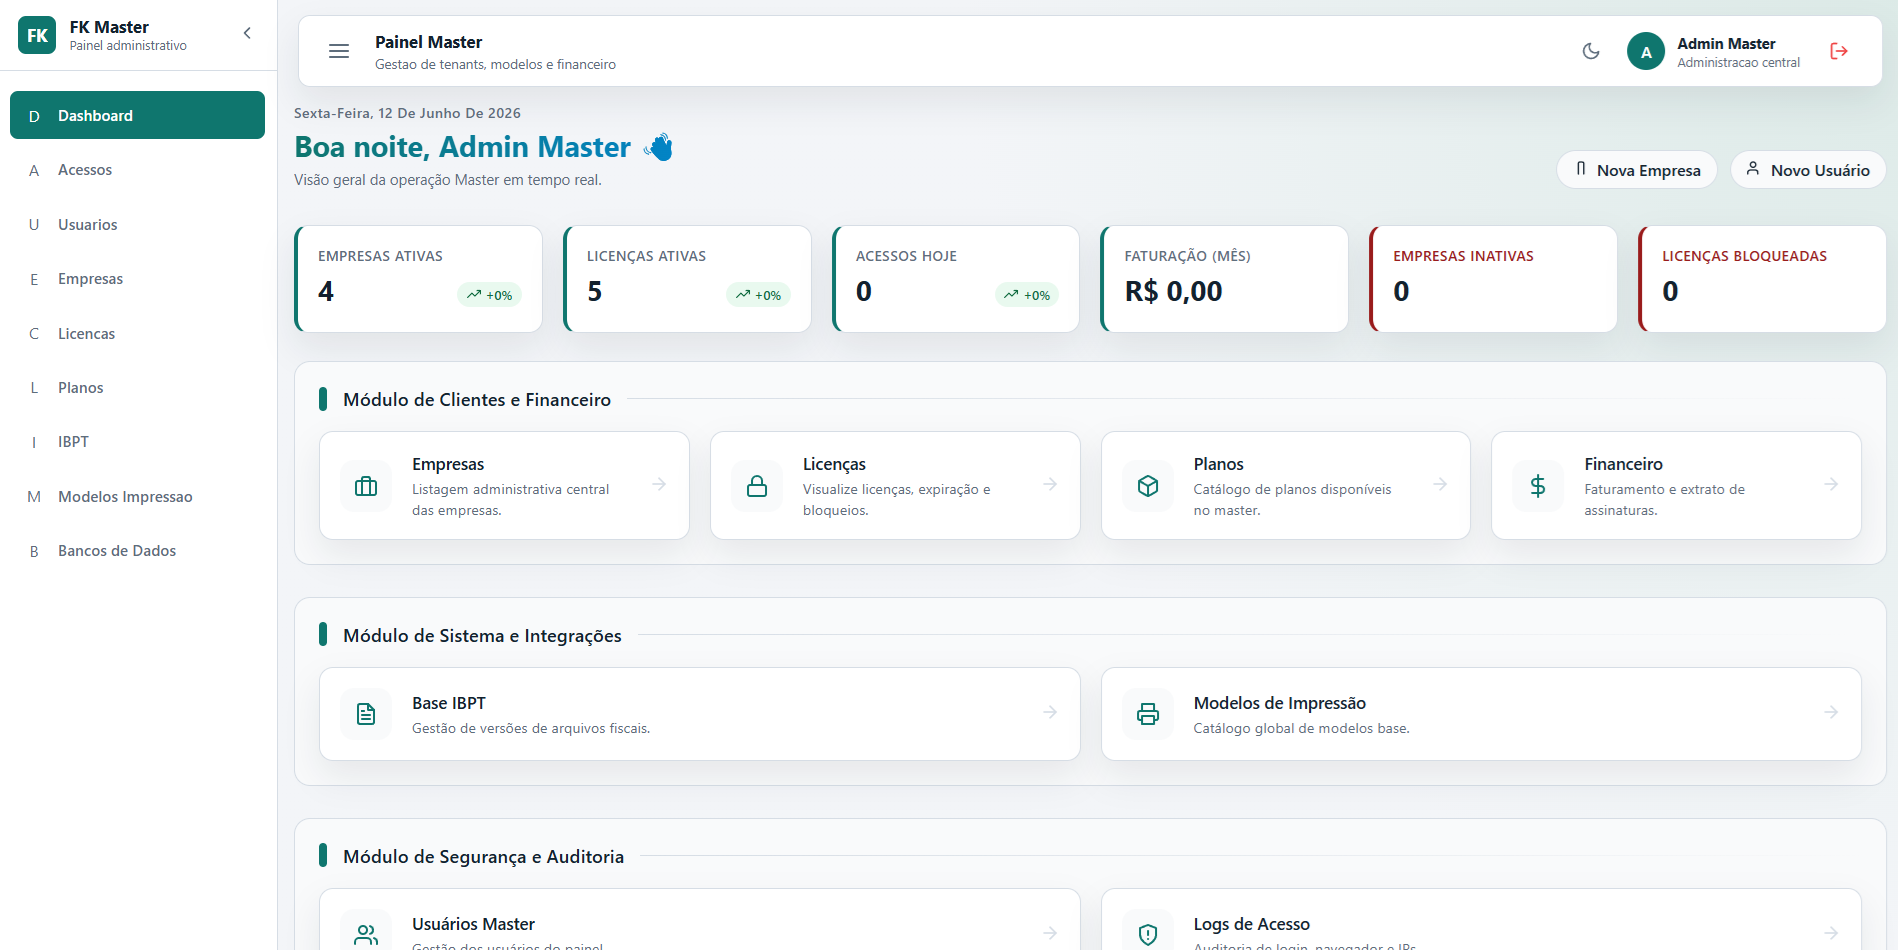
\includegraphics[width=0.95\textwidth]{figuras/05-desenvolvimento/daschboard.png}
    \legend{Fonte: Própria do autor (2026).}
\end{figure}

A interface ilustrada na \autoref{fig:dashboard_interface} foi concebida para minimizar
o tempo de detecção de anomalias (\textit{Mean Time To Detect} -- MTTD),
organizando os indicadores de maior criticidade operacional em posição de
destaque visual. Esta decisão de design reflete um princípio de UX para
ferramentas de monitoramento: a hierarquia visual deve corresponder à hierarquia
de impacto no negócio.

\subsection{Arquitetura Reativa da Interface e Estratégia de Atualização}

A escolha do \textit{Vue.js} 3 como \textit{framework} de interface não foi
arbitrária. O sistema de reatividade baseado em \textit{Proxy} da \textit{Composition
API} do Vue 3, em contraste com o sistema de observadores (\textit{watchers})
do Vue 2, oferece granularidade de reatividade por propriedade, reduzindo
re-renderizações desnecessárias em componentes que exibem grandes volumes de
dados de telemetria. A interface é composta por componentes desacoplados,
cada um responsável por um domínio de KPI específico, e se comunica com a API
Central via cliente HTTP baseado em \textit{Axios}, com estratégia de polling
configurável para atualização periódica dos indicadores sem necessidade de
recarregamento de página.


% ------------------------------------------------------------------------------
\section{Demonstração das Interfaces de Gestão e Evidências}
% ------------------------------------------------------------------------------

A implementação das interfaces de gestão do Hub Master constitui a materialização
dos requisitos funcionais e não-funcionais descritos nas seções anteriores.
Cada tela foi projetada como uma camada de abstração sobre operações técnicas
complexas, tornando acessíveis ao operador ações que, em sua essência,
envolvem manipulação de infraestrutura de banco de dados e controle de acesso
multi-tenant.

\subsection{Acesso e Gestão de Usuários}

O acesso à plataforma é protegido por uma camada de autenticação robusta
(\autoref{fig:login_master}), integrada ao \textit{Laravel Sanctum}. O Sanctum
fornece autenticação baseada em tokens API de forma simplificada, adequada para
aplicações SPA como a desenvolvida. A gestão de usuários é dividida entre usuários
administrativos do sistema (\autoref{fig:criacao_usuario_master}) e usuários
específicos de cada oficina parceira (\autoref{fig:criacao_usuario_empresa}).

\begin{figure}[htb]
    \caption{\label{fig:login_master}Interface de Autenticação do Hub Master}
    \centering
    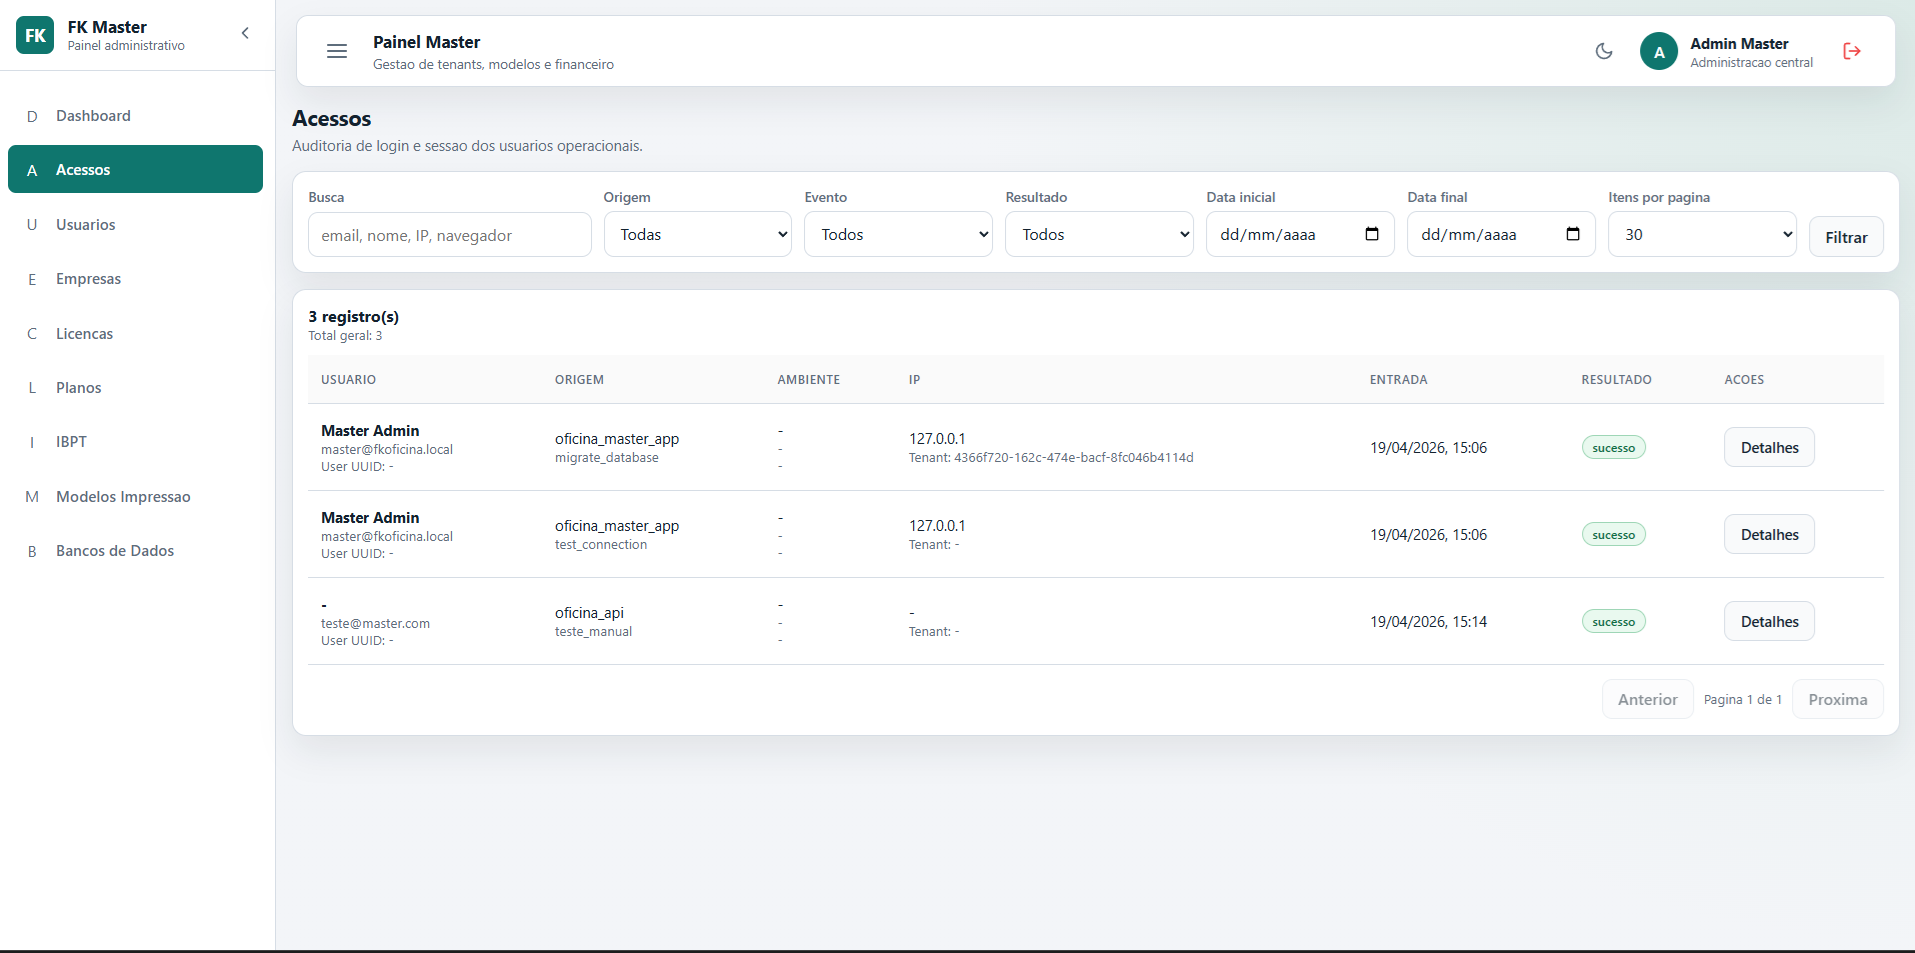
\includegraphics[width=0.85\textwidth]{figuras/05-desenvolvimento/aceso_user.png}
    \legend{Fonte: Própria do autor (2026).}
\end{figure}

\begin{figure}[htb]
    \centering
    \subfloat[Criação de Usuário Master]{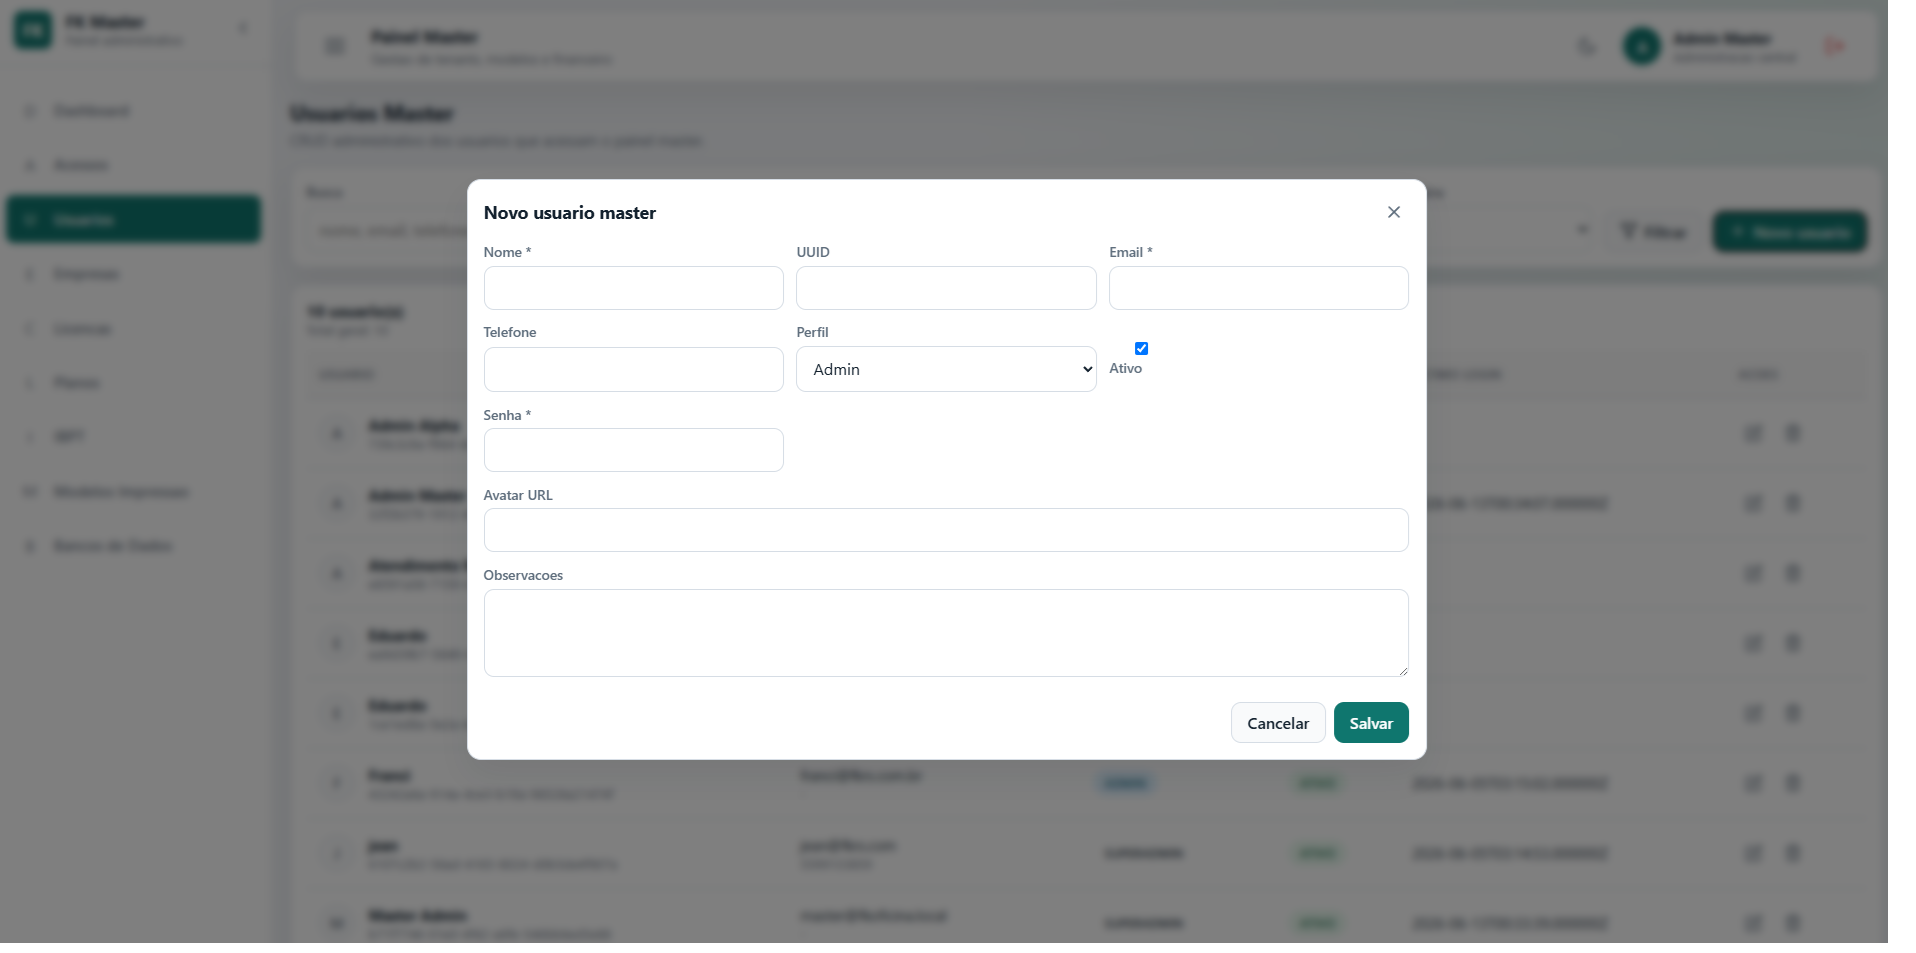
\includegraphics[width=0.95\textwidth]{figuras/05-desenvolvimento/criacao_usuario_master.png}\label{fig:criacao_usuario_master}}
    \\
    \subfloat[Criação de Usuário de Empresa]{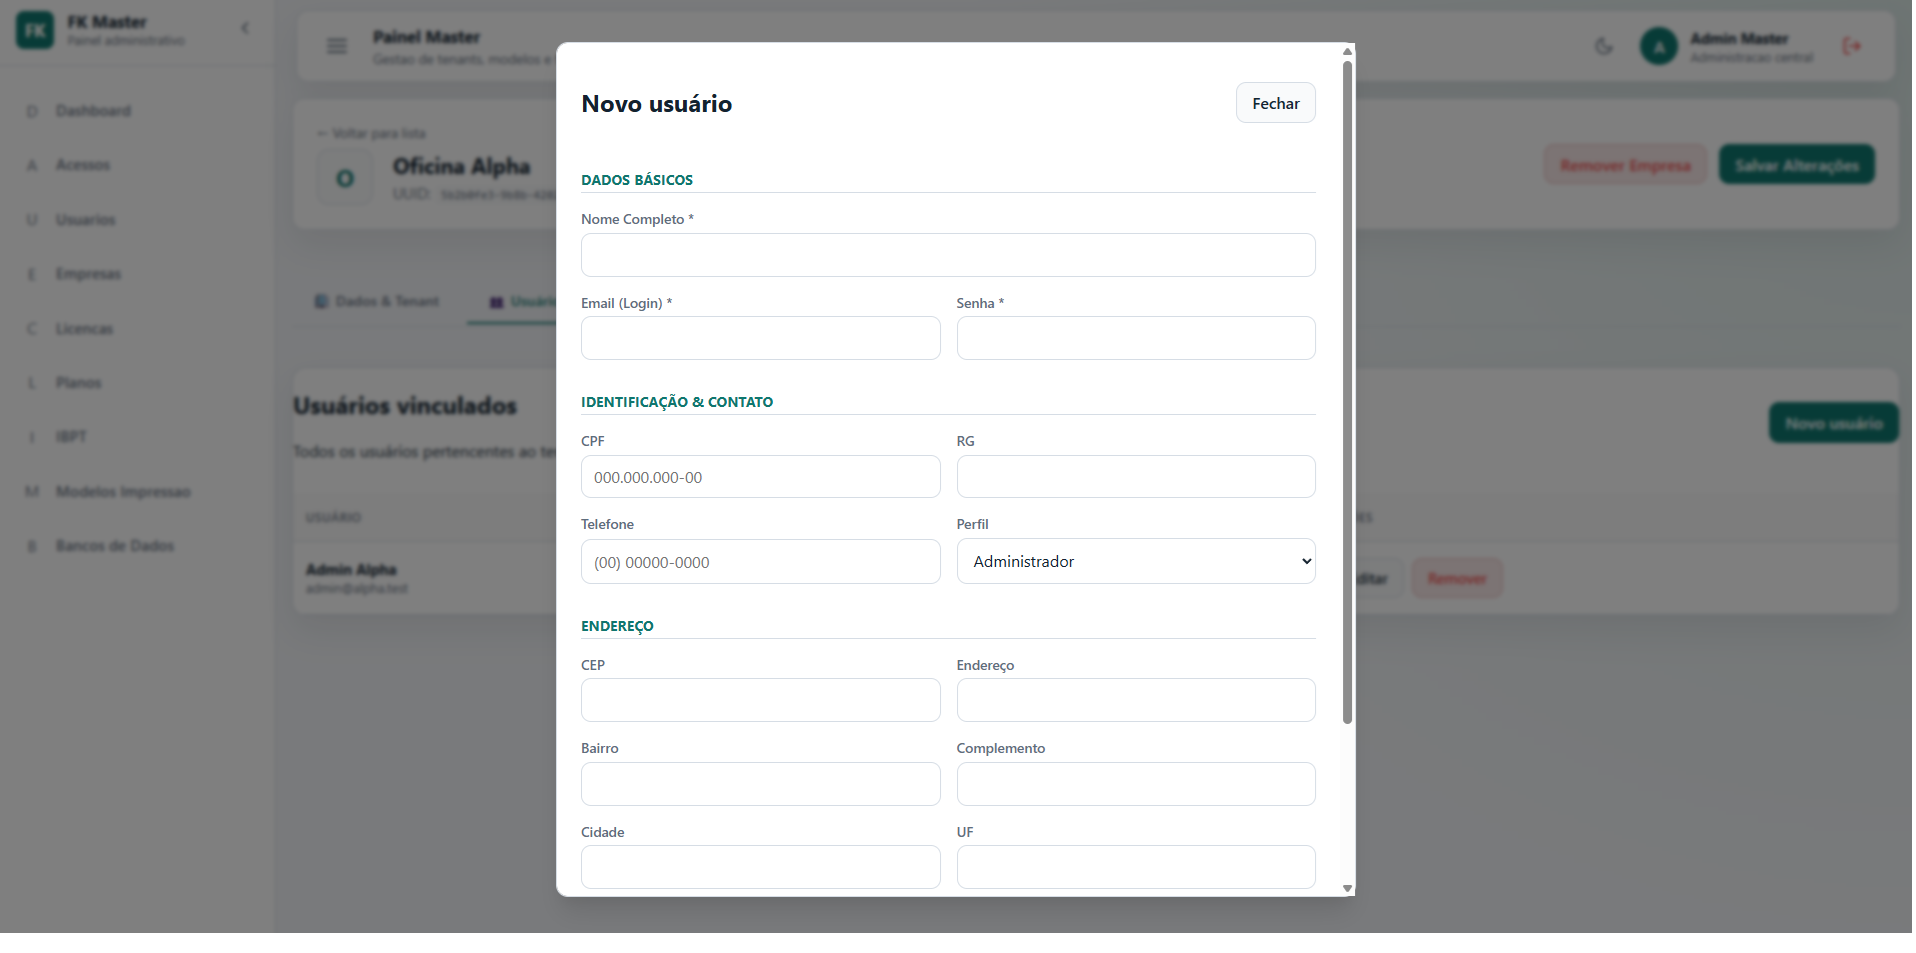
\includegraphics[width=0.95\textwidth]{figuras/05-desenvolvimento/criacao_usuario_empresa.png}\label{fig:criacao_usuario_empresa}}
    \caption{Interfaces de Gestão de Usuários e Controle de Acesso}
    \legend{Fonte: Própria do autor (2026).}
\end{figure}

\begin{figure}[htb]
    \caption{\label{fig:lista_usuarios}Listagem Geral de Usuários Cadastrados no Sistema}
    \centering
    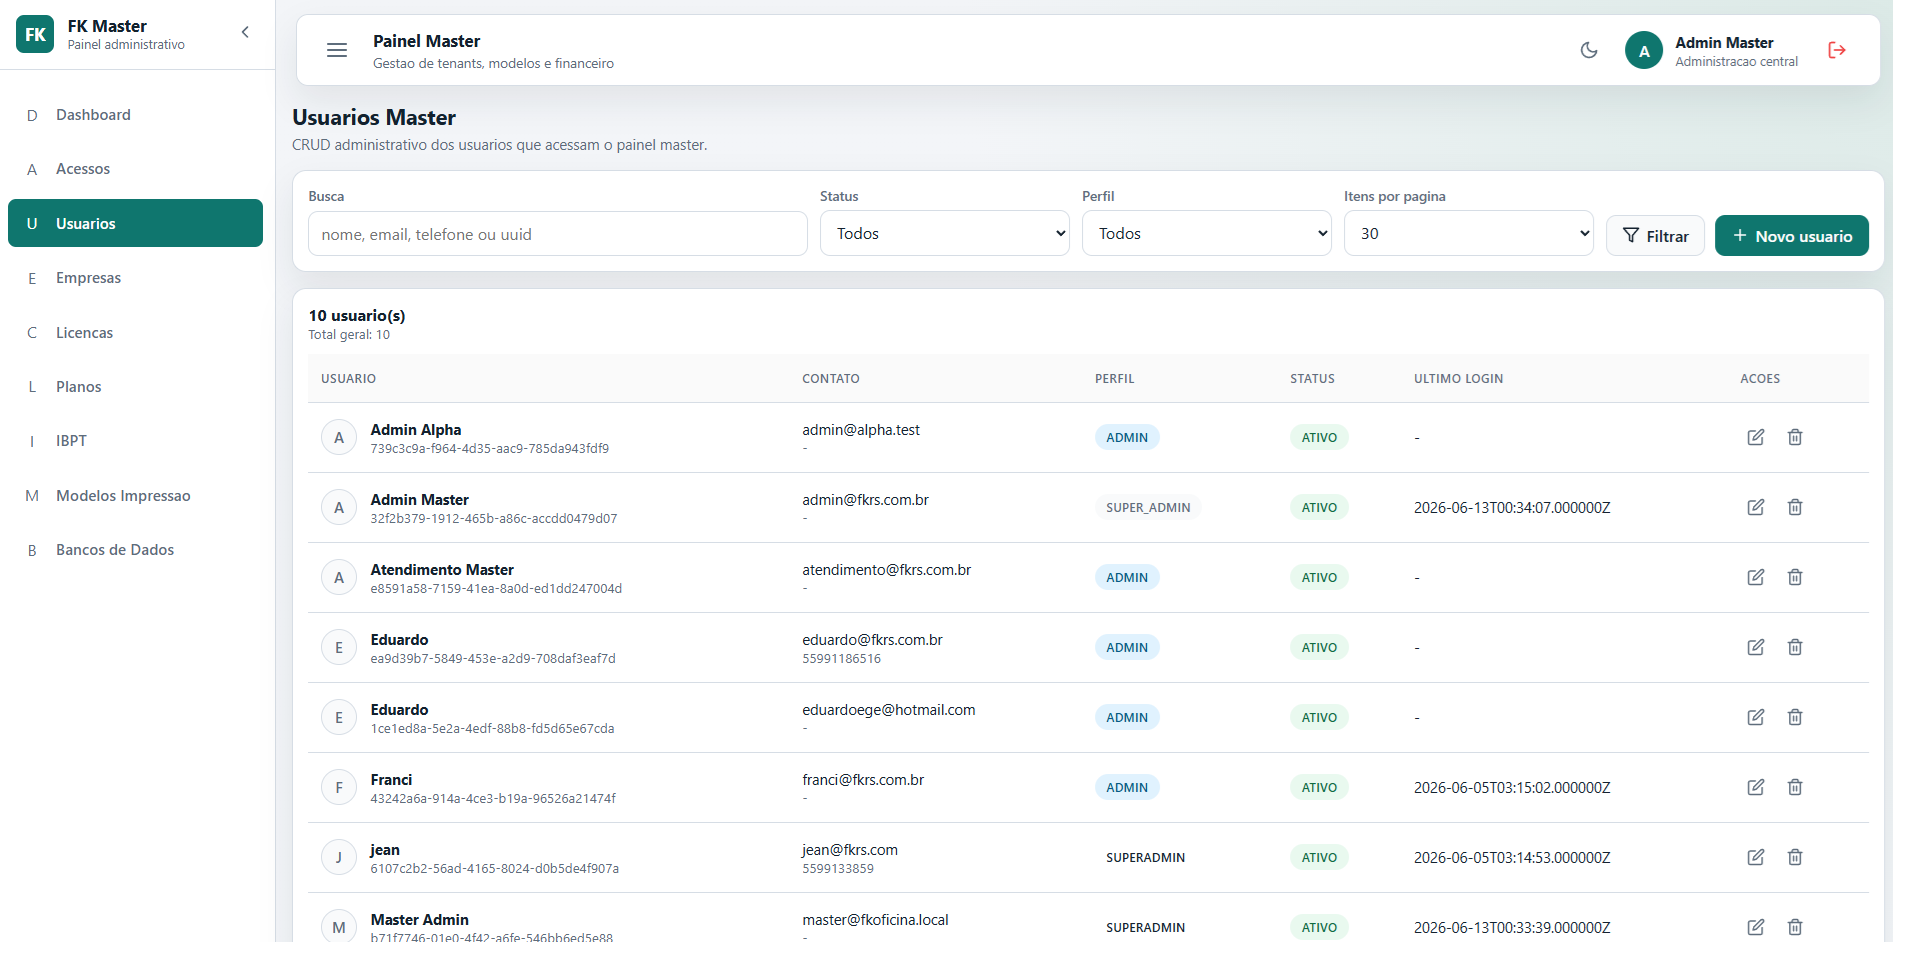
\includegraphics[width=0.95\textwidth]{figuras/05-desenvolvimento/lista de usuarios cadastrados.png}
    \legend{Fonte: Própria do autor (2026).}
\end{figure}

\subsection{Gestão de Tenants, Planos e Licenciamento}

A gestão individual de cada cliente é viabilizada pela interface de listagem
de \textit{tenants} (\autoref{fig:lista_tenants_interface}). O administrador obtém,
em uma única visão, o status operacional de cada banco de dados (\autoref{fig:lista_bancos})
e a validade das licenças correspondentes. A flexibilidade comercial é garantida
pelas interfaces de criação de planos (\autoref{fig:criacao_plano}) e emissão de
licenças (\autoref{fig:criacao_licença}), que permitem configurar dinamicamente
os recursos disponíveis para cada oficina.

\begin{figure}[htb]
    \caption{\label{fig:lista_tenants_interface}Listagem Geral de Empresas Cadastradas}
    \centering
    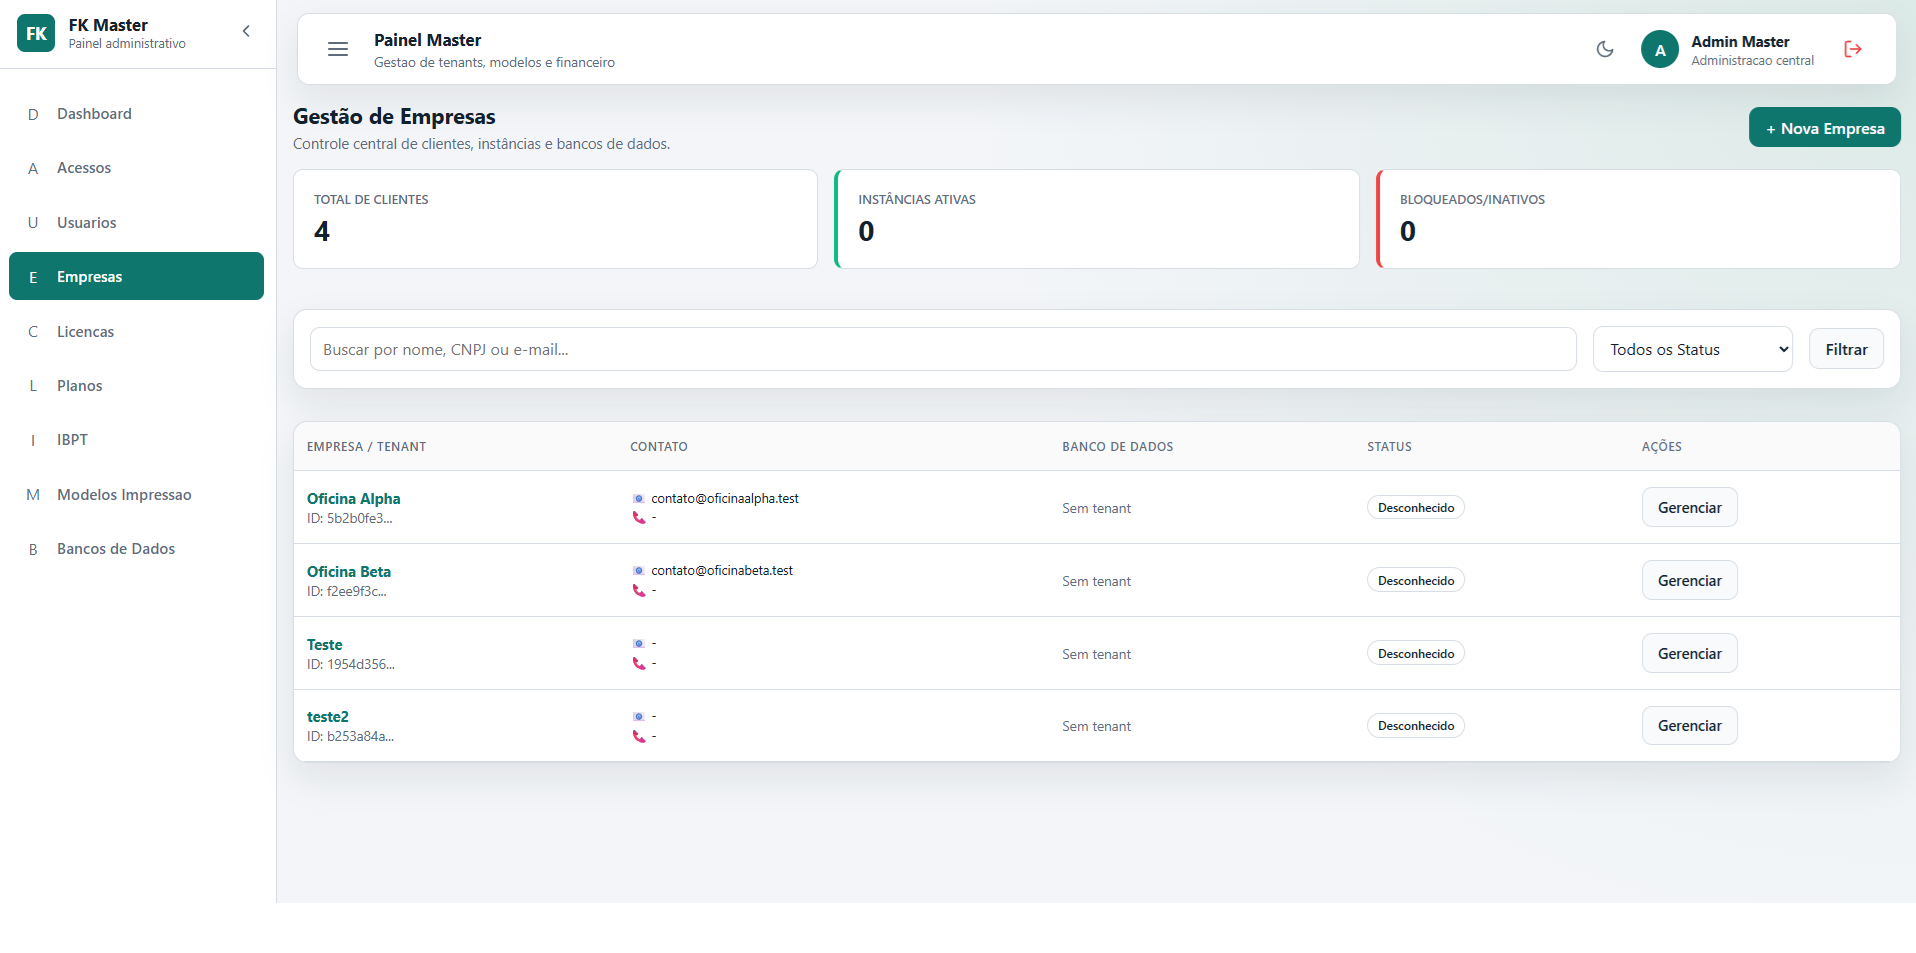
\includegraphics[width=0.95\textwidth]{figuras/05-desenvolvimento/lista_empresas.png}
    \legend{Fonte: Própria do autor (2026).}
\end{figure}

\begin{figure}[htb]
    \caption{\label{fig:lista_bancos}Monitoramento de Instâncias de Bancos de Dados}
    \centering
    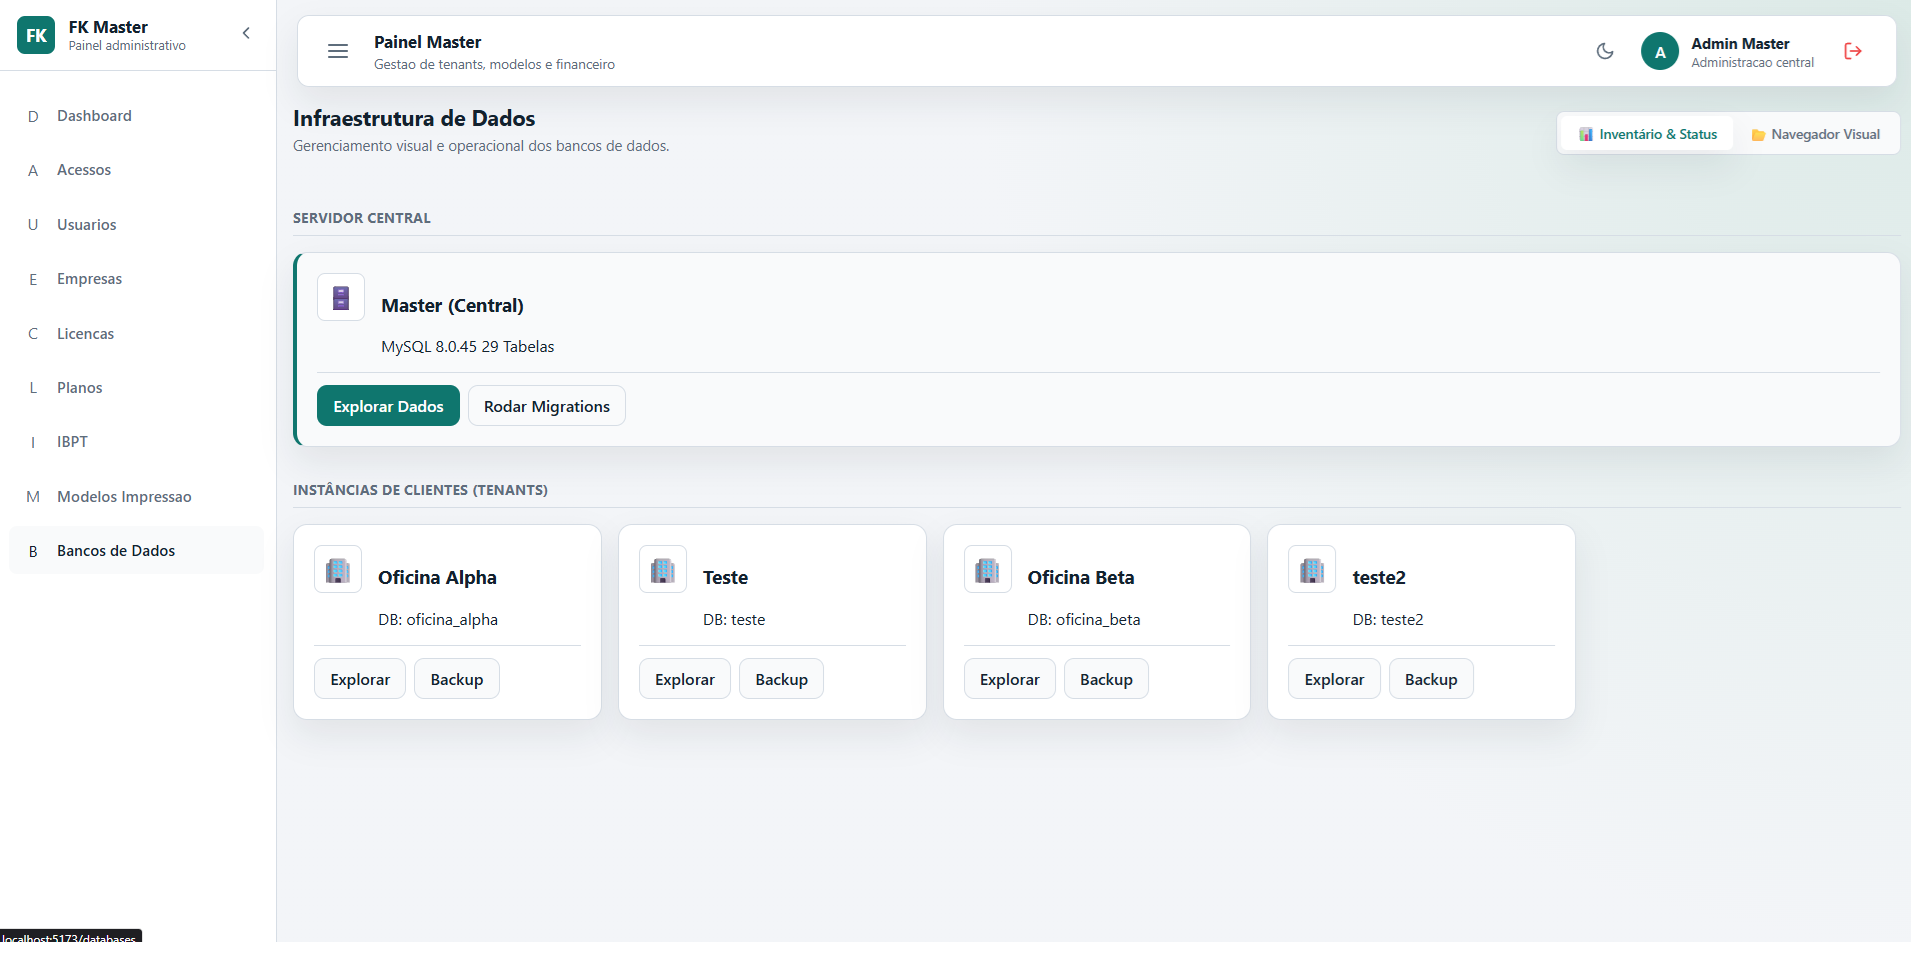
\includegraphics[width=0.95\textwidth]{figuras/05-desenvolvimento/lista_bancos.png}
    \legend{Fonte: Própria do autor (2026).}
\end{figure}

\begin{figure}[htb]
    \centering
    \subfloat[Listagem de Planos]{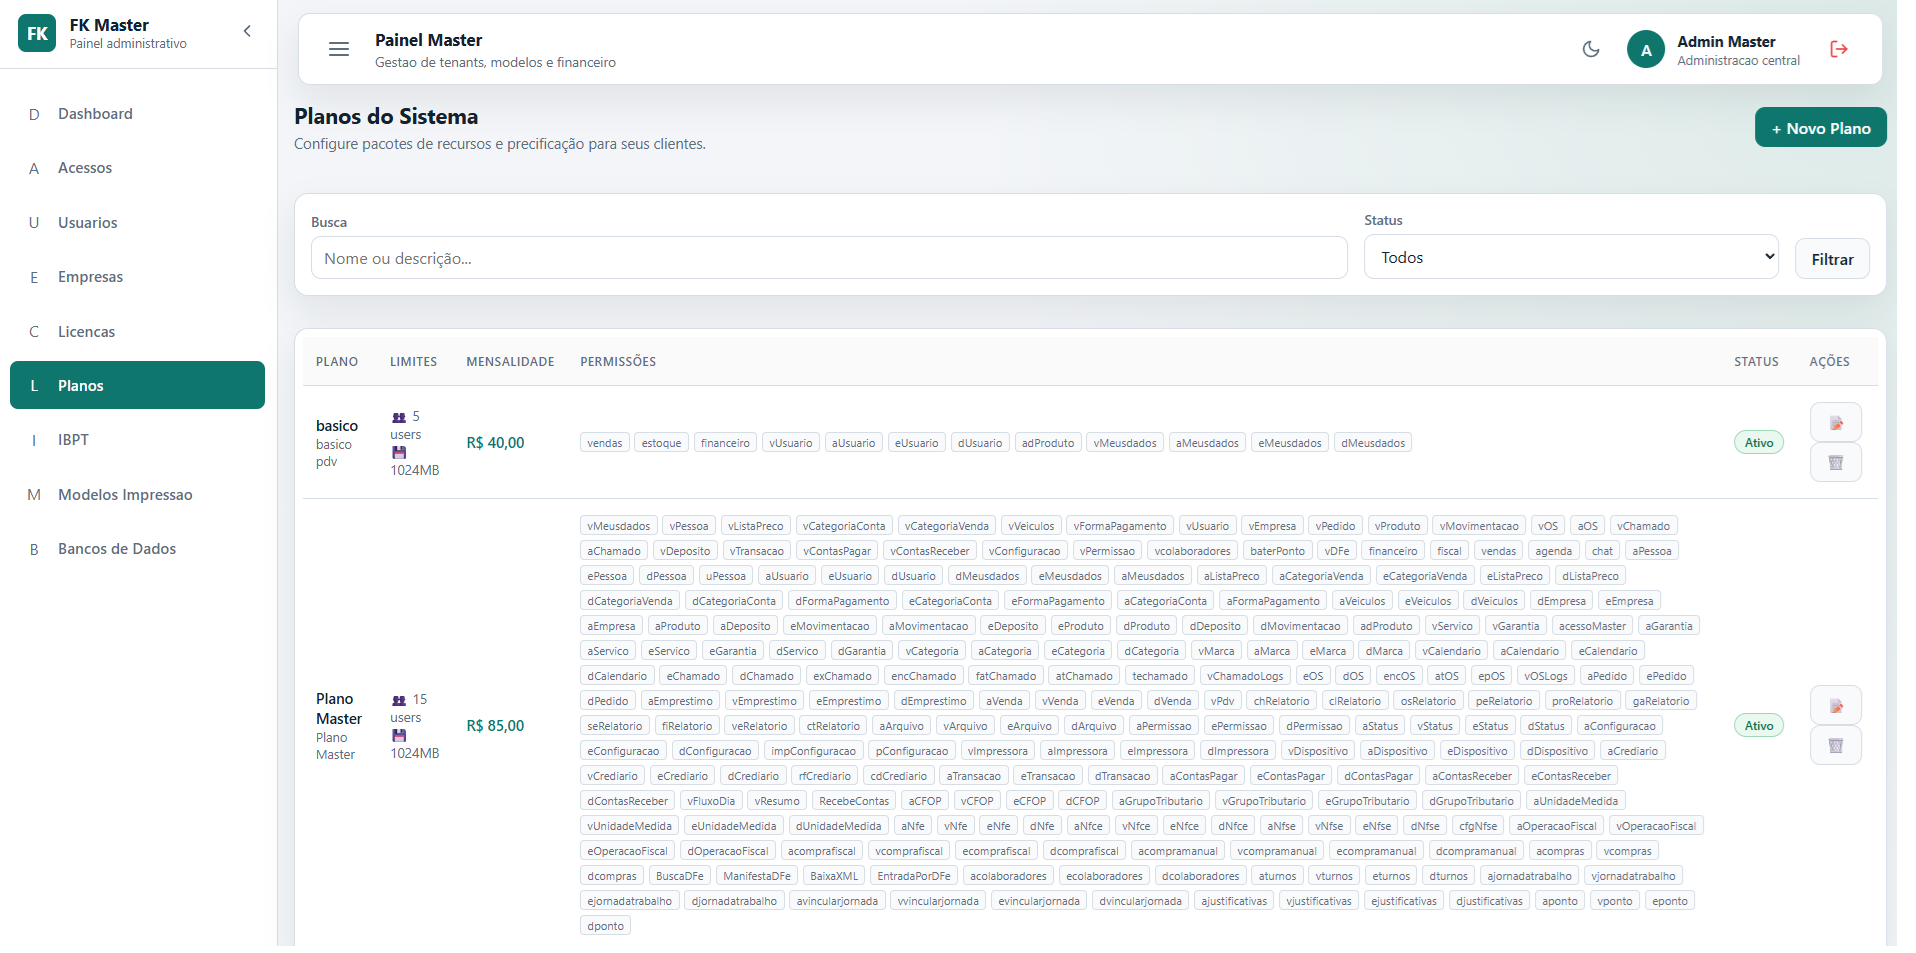
\includegraphics[width=0.95\textwidth]{figuras/05-desenvolvimento/listas_planos.png}\label{fig:listas_planos}}
    \\
    \subfloat[Listagem de Licenças]{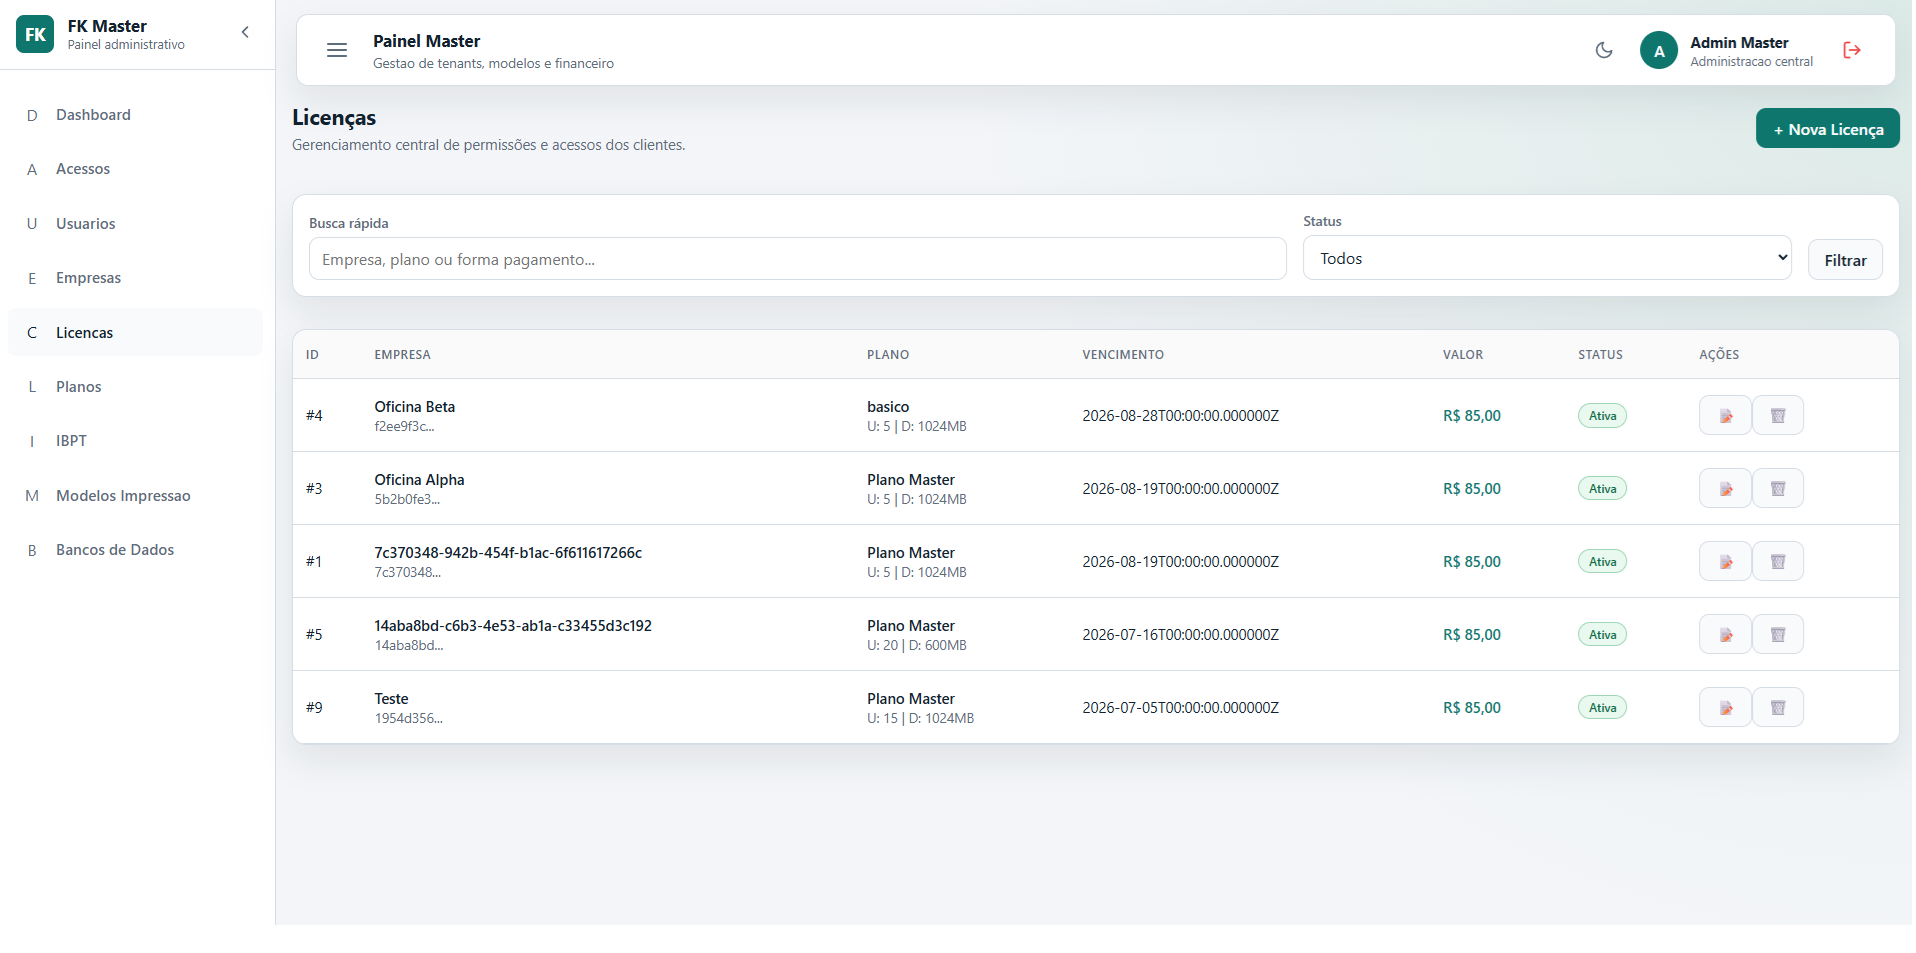
\includegraphics[width=0.95\textwidth]{figuras/05-desenvolvimento/listas_licenças.png}\label{fig:listas_licenças}}
    \caption{Visualização Consolidada de Planos e Licenças no Ecossistema}
    \legend{Fonte: Própria do autor (2026).}
\end{figure}

\begin{figure}[htb]
    \centering
    \subfloat[Criação de Planos]{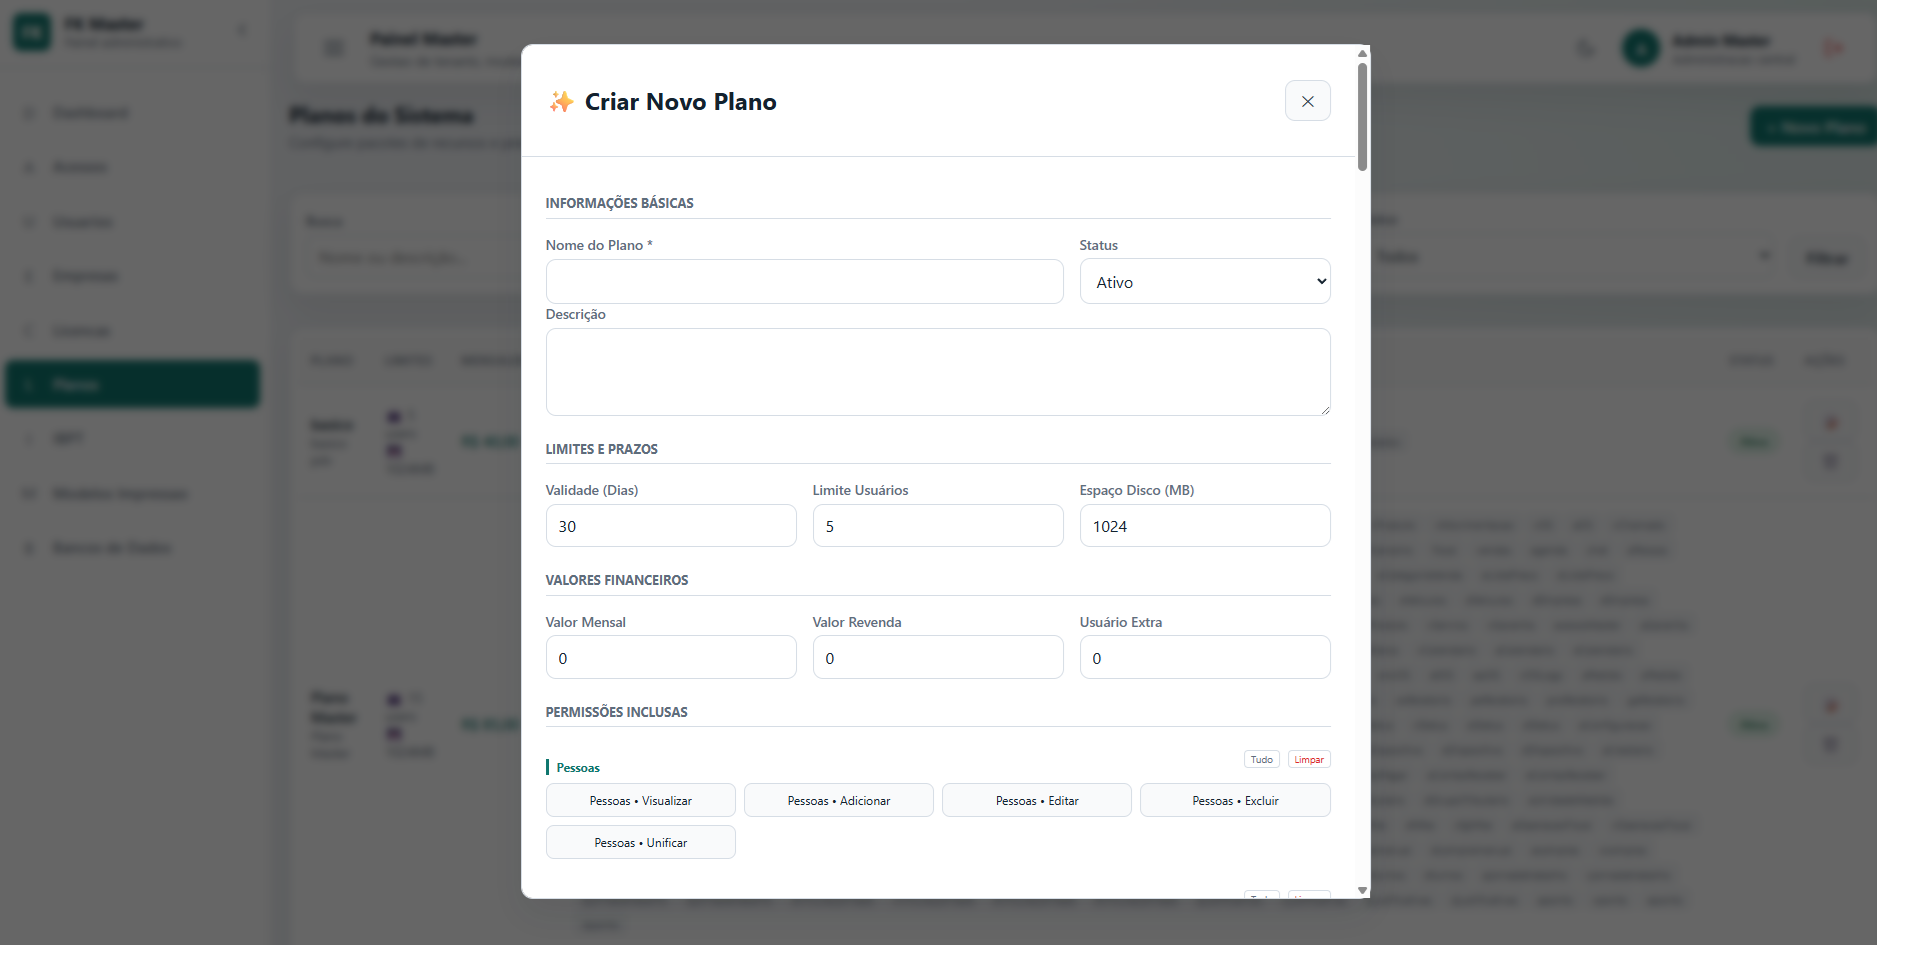
\includegraphics[width=0.95\textwidth]{figuras/05-desenvolvimento/criacao_plano.png}\label{fig:criacao_plano}}
    \\
    \subfloat[Emissão de Licença]{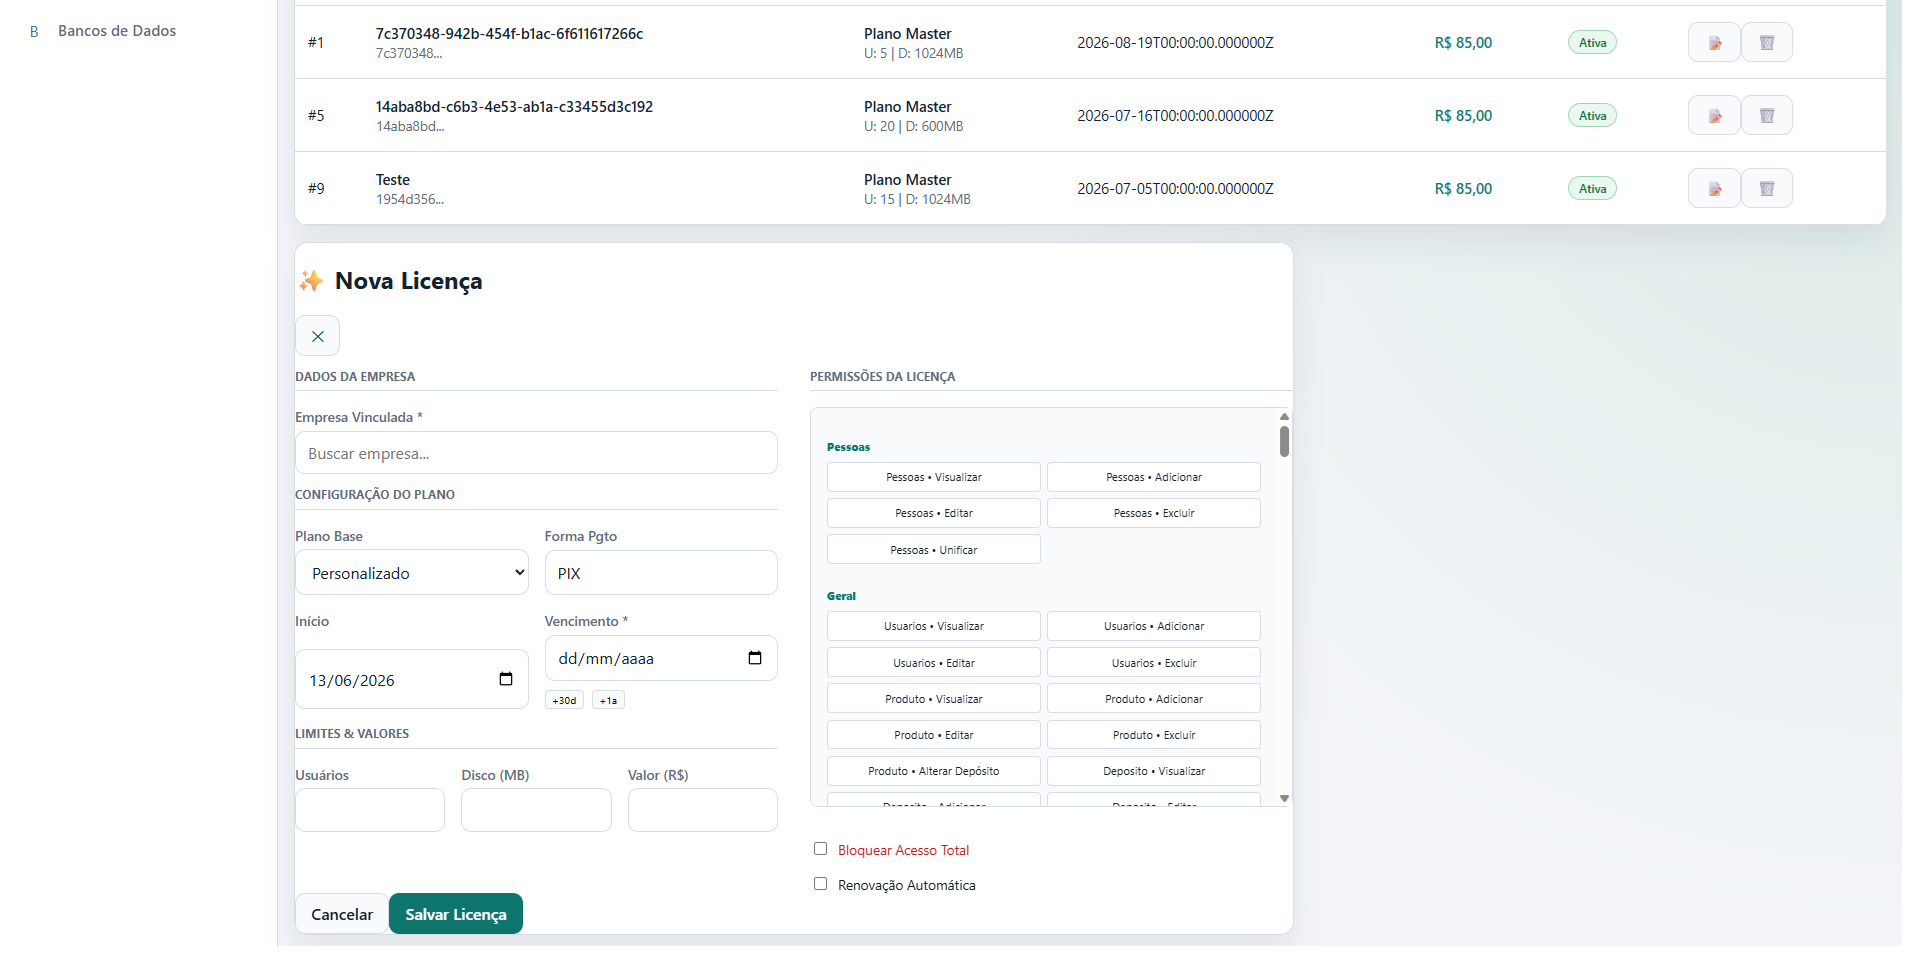
\includegraphics[width=0.95\textwidth]{figuras/05-desenvolvimento/criacao_licença.png}\label{fig:criacao_licença}}
    \caption{Interfaces de Configuração Comercial e Emissão de Licenças}
    \legend{Fonte: Própria do autor (2026).}
\end{figure}

\begin{figure}[htb]
    \caption{\label{fig:alteracao_plano_interface}Interface de Alteração e Ajuste de Plano de Empresa}
    \centering
    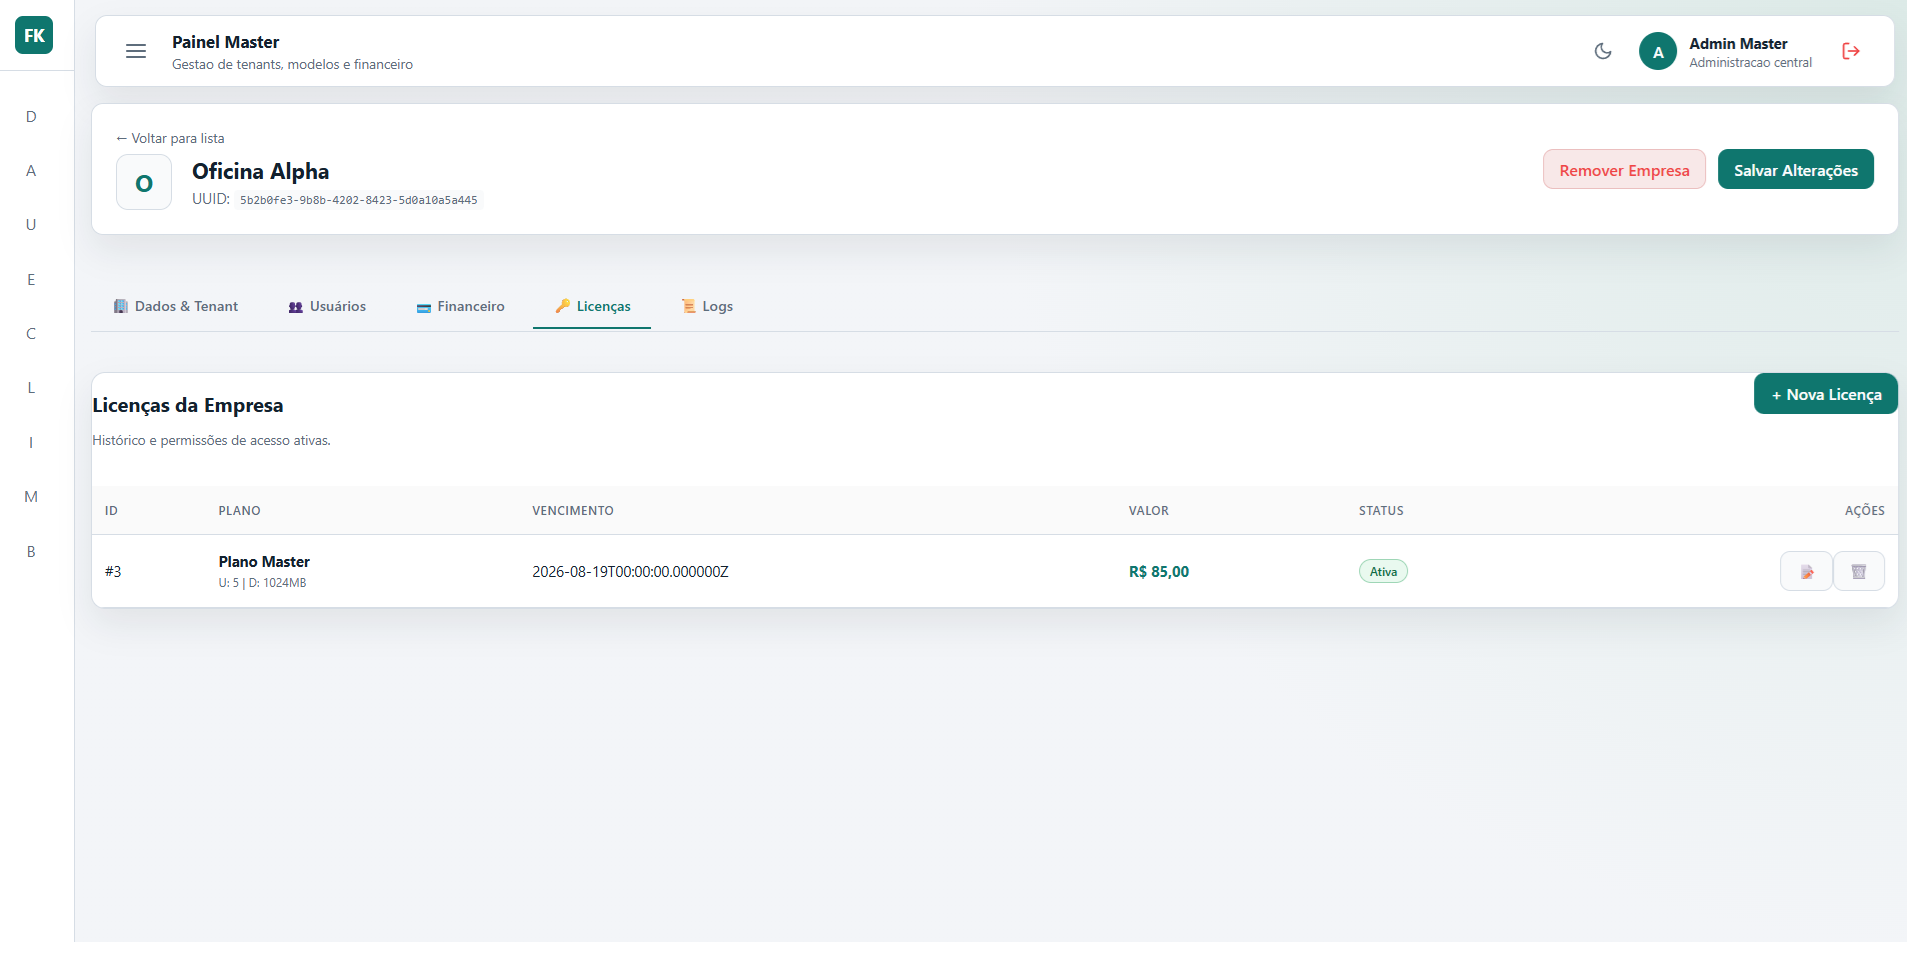
\includegraphics[width=0.95\textwidth]{figuras/05-desenvolvimento/alteração_plano_empresa.png}
    \legend{Fonte: Própria do autor (2026).}
\end{figure}

\subsection{Evidências de Desenvolvimento e Controle de Versão}

O código-fonte integral encontra-se disponível no repositório registrado no
Apêndice~\ref{apx:repositorio}. A análise deste registro permite verificar a
autoria e a consistência das contribuições, constituindo um registro auditável
do processo de engenharia aplicado. A transição entre as fases de pesquisa,
prototipação e implementação final é visível no histórico de commits, validando
a metodologia descrita anteriormente.

Esta camada de gestão visual e documental é o que eleva o Oficina Master da categoria de
ferramenta técnica de automação à de plataforma estratégica de gestão de
ecossistemas SaaS: ao abstrair a complexidade dos mecanismos técnicos em uma
experiência de usuário coerente, o sistema habilita que decisões de infraestrutura
e negócio sejam tomadas com base em evidências em tempo real.
